\documentclass[11pt, a4paper]{report}
\usepackage{graphicx}
\usepackage[table,xcdraw]{xcolor}
\usepackage{geometry}
\usepackage{float}
\usepackage{authblk}
\usepackage{anyfontsize}
\usepackage[document]{ragged2e}
\usepackage{titlesec}
\usepackage[parfill]{parskip}
\usepackage{color}   %May be necessary if you want to color links
\usepackage{hyperref}
\usepackage{caption}
\usepackage{longtable}
\usepackage{blindtext}
\usepackage{pdfpages}
\usepackage[backend=biber]{biblatex}
\hypersetup{
    colorlinks=true, %set true if you want colored links
    linktoc=all,     %set to all if you want both sections and subsections linked
    linkcolor=black,  %choose some color if you want links to stand out
}
\titleformat{\chapter}[hang]
{\normalfont\huge\bfseries}{\chaptertitlename\ \thechapter}{1em}{} 
\geometry{left=2.5cm,right=2.5cm,top=2.5cm,bottom=2.5cm}
\graphicspath{ {./images/} }

\begin{document}  

\pagestyle{empty}
\centering
\fontsize{2cm}{2cm}\selectfont{Module Design Document} \\
\vspace{2mm}
\fontsize{1cm}{1cm}\selectfont Audio digital signal processor \\
\vspace{2mm}
\large BeCreative Minor\\
\normalsize
\vspace{4cm}
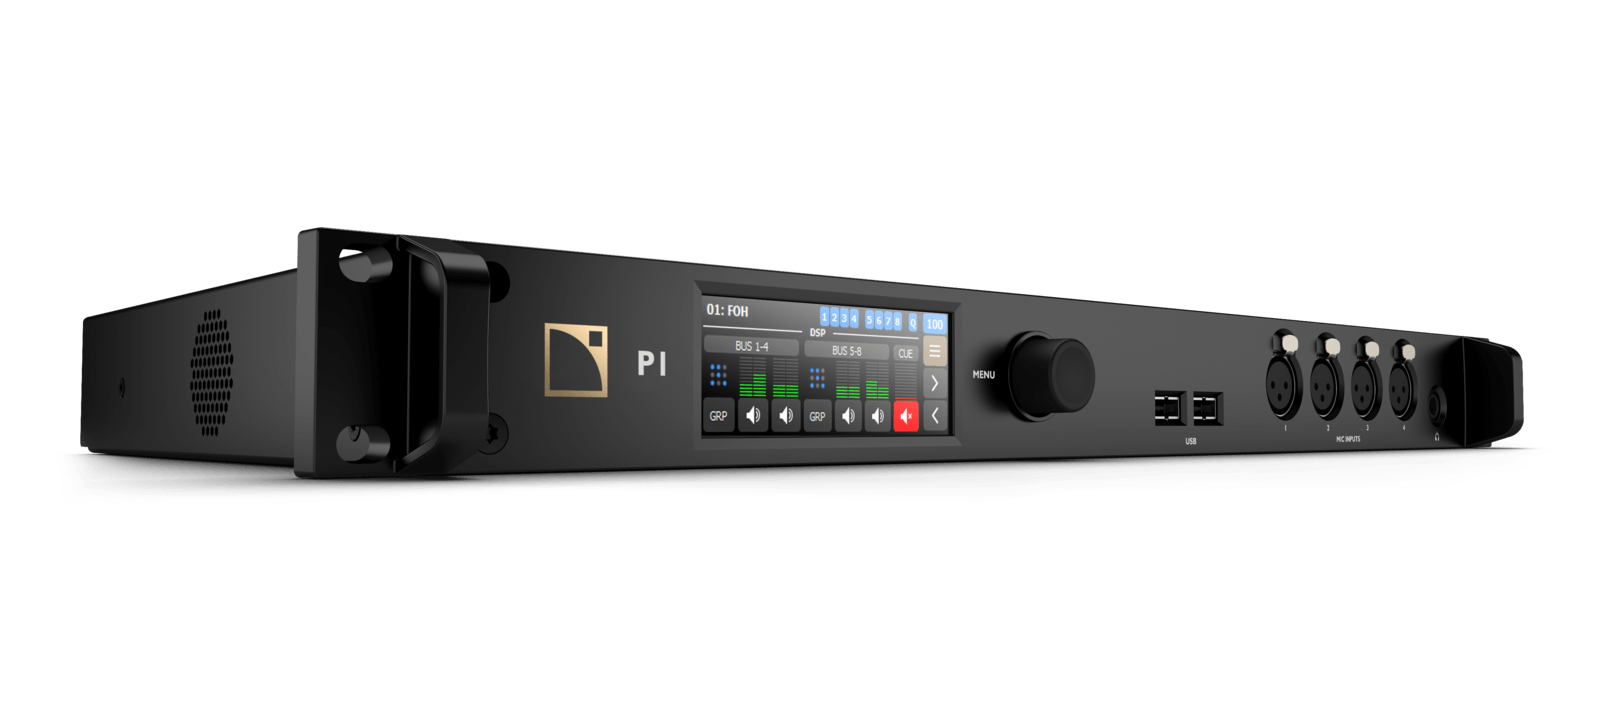
\includegraphics[width=\linewidth]{3DR_P1_Perspective.png}\\
\vfill
\normalsize Busse Lommers \\
Robin van den Dungen \\
Mahmud Gürler \\
Silas Kamphuis \\
Hein Verhallen \\
Youri Tils \\
Fontys Hogescholen, De Rondom 1, 5612 AP Eindhoven \\
\today

\begin{justify}

%\chapter*{Summary}

\newpage
\tableofcontents
\thispagestyle{empty}

\listoffigures
\thispagestyle{empty}


\listoftables
\thispagestyle{empty}

\newpage
\pagestyle{plain}
\setcounter{page}{1}

\chapter*{Abbreviation List}

\begin{table}[!h]
	\centering
\begin{tabular}{|c|c|}
	\hline
\textbf{Abbreviation} & \textbf{Explanation}        \\ \hline
DSP 					& Digital Signal Processor    \\ \hline
ADC 					& Analog-to-Digital Converter \\ \hline
DAC 					& Digital-to-Analog Converter \\ \hline
RAM 					& Random access memory	    \\ \hline
SINAD 					& Signal to noise and distortion \\ \hline
TRS 					& Tip ring sleeve connector (jack) \\ \hline
FPGA 					& Field programmable gate array \\ \hline
CH 						& Channel					\\ \hline
FFT 					& Fast Fourier Transform	\\ \hline
BPF 					& Band-Pass Filter			\\ \hline

\end{tabular}
\caption{List of commonly used Abbreviations}
\label{Abbreviation list}
\end{table}


    %\pagestyle{empty}
\centering
\fontsize{2cm}{2cm}\selectfont{Module Design Document} \\
\vspace{2mm}
\fontsize{1cm}{1cm}\selectfont Audio digital signal processor \\
\vspace{2mm}
\large BeCreative Minor\\
\normalsize
\vspace{4cm}
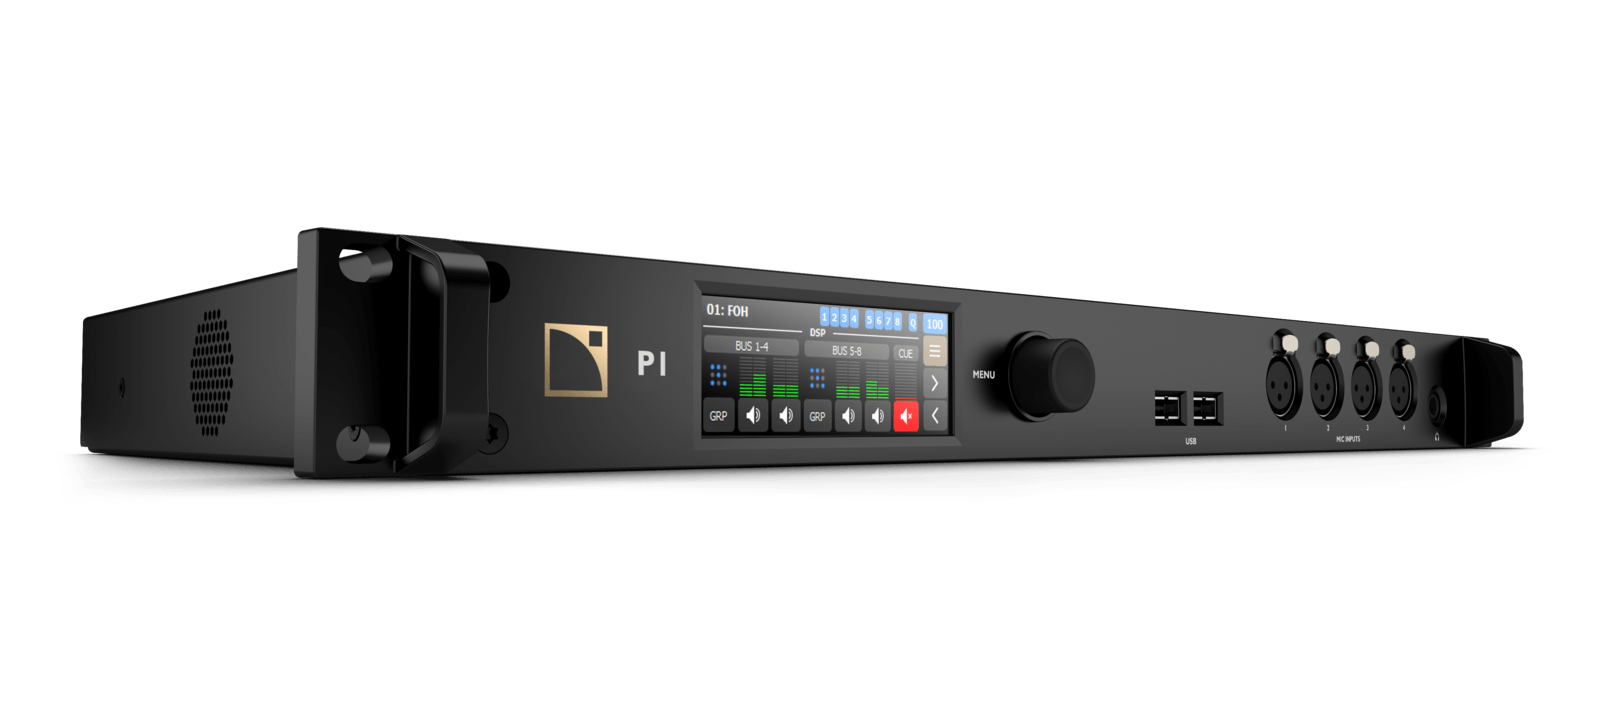
\includegraphics[width=\linewidth]{3DR_P1_Perspective.png}\\
\vfill
\normalsize Busse Lommers \\
Robin van den Dungen \\
Mahmud Gürler \\
Silas Kamphuis \\
Hein Verhallen \\
Youri Tils \\
Fontys Hogescholen, De Rondom 1, 5612 AP Eindhoven \\
\today

\begin{justify}

\chapter*{Summary}
The following text translates to English as:

This report describes how this project group created an audio DSP for the BeCreative Minor. This was done because the members of the group wanted to learn more about it and improve their technical knowledge.

Chapter "Problem Description" outlines the project's background and goals. Chapter "Research" describes the preliminary investigations conducted. Chapter "Concept Development" explains how the product concept was developed. Chapter "Realization" details the actual design of the audio DSP. Chapter "Verification" discusses the product testing process. Finally, in chapters "Conclusions" and "Recommendations," the conclusion and recommendations are respectively described.

\newpage
\tableofcontents
\thispagestyle{empty}

\listoffigures
\thispagestyle{empty}

\listoftables
\thispagestyle{empty}

\newpage
\pagestyle{plain}

\chapter*{Report contribution}	%Fill-in only regarding the report contribution.
\begin{longtable}{|c|c|c|}
	\hline
	\textbf{Chapter} & \textbf{Paragraph} & \textbf{Person} \\ \hline
	Problem Description			& Background					& All	 					\\ \hline
	Introduction				& NA							& Busse 					\\ \hline
								& Problem description			& Robin						\\ \hline
								& Project goals					& All						\\ \hline
								& Requirements					& All 						\\ \hline
								& Project scope					& All 						\\ \hline
								& Boundary condition			& All						\\ \hline
								& Project approach				& All						\\ \hline
								& Verification method			& All						\\ \hline
	Research 					& Research objectives			& All 						\\ \hline
								& Research questions			& All 						\\ \hline
								& Research approach				& All 						\\ \hline
								& Results						& All 						\\ \hline
	Concept Development 		& Concept overview				& Youri						\\ \hline
								& Front-end						& Silas						\\ \hline
								& Audio-DSP						& Youri						\\ \hline
								& Back-end						& Silas						\\ \hline
								& Interfacing					& Robin						\\ \hline
								& Front-end						& Robin						\\ \hline
								& Audio-DSP						& Youri						\\ \hline
								& Back-end						& Robin						\\ \hline
								& Power supplies				& Mahmud \& Robin			\\ \hline
								& Modules						& Busse						\\ \hline
								& UI							& Hein \& Busse				\\ \hline
								& Hardware programming			& Busse						\\ \hline
								& Hardware design				& Busse						\\ \hline
								& Design decissions				& Busse						\\ \hline
	Realization					& Hardware						& NA						\\ \hline
								& Schematic						& Robin						\\ \hline
								& Printed circuit board			& Silas						\\ \hline
								& Case							& Busse						\\ \hline
								& Firmware						& Youri						\\ \hline
								& I2S decoder and encoder		& Youri						\\ \hline
								& I2C controller				& Youri						\\ \hline
								& Band-pass filter				& Youri						\\ \hline
								& Sinewave generator			& Youri						\\ \hline
								& Effects						& Youri \& Busse			\\ \hline
								& User interface				& Hein \& Busse				\\ \hline
								& User interface				& Hein \& Busse				\\ \hline
	Verification				& Method						& Robin						\\ \hline
								& Hardware						& Mahmud \& Robin			\\ \hline
								& Firmware						& Youri						\\ \hline
								& Results						& NA						\\ \hline
								& Hardware						& Mahmud					\\ \hline
								& Firmware						& Youri						\\ \hline
								& Conclusions					& Mahmud \& Silas \& Robin 	\\ \hline
								& Hardware						& Mahmud					\\ \hline
								& Firmware						& Youri						\\ \hline
	Conclusions					& NA							& Silas						\\ \hline
	Recommendations				& NA							& Silas						\\ \hline
	Summary						& NA							& Robin						\\ \hline
	Bibliography				& NA							& Busse						\\ \hline
	Appendix A: State-space		& NA							& Youri						\\ \hline
	Appendix B: VHDL code		& I2S decoder					& Youri						\\ \hline
								& I2S encoder					& Youri						\\ \hline
								& I2C master					& Youri						\\ \hline
								& State-space BPF code			& Youri						\\ \hline
								& Sinewave generator code		& Youri						\\ \hline
	Appendix C: Schematics		& Buck converter schematic		& Mahmud					\\ \hline
								& SEPIC schematic				& Silas						\\ \hline
								& Linear regulator schematic	& Silas	\& Robin			\\ \hline
								& Main board schematic			& Robin						\\ \hline
								& Buck converter calculations	& Silas						\\ \hline
								& SEPIC calculations			& Robin						\\ \hline
	Appendix D: UI design		& Main menu						& Busse						\\ \hline
								& Adjust preset menu			& Busse						\\ \hline
	Appendix E: Case			& Top view						& Busse						\\ \hline
								& Front view					& Busse						\\ \hline
								& Rear view						& Busse						\\ \hline
	Appendix F: Verification	& Ground spring					& Robin						\\ \hline

	\caption{Revision list of the document}
	\label{table:revision_history}
\end{longtable}

\newpage
\pagestyle{plain}
\setcounter{page}{1}

\chapter*{Abbreviation List}

\begin{table}[!h]
	\centering
	\begin{tabular}{|c|c|}
		\hline
		\textbf{Abbreviation} & \textbf{Explanation}	\\ \hline
		DSP 					& Digital Signal Processor    				\\ \hline
		ADC 					& Analog-to-Digital Converter 				\\ \hline
		BPF 					& Band-Pass Filter							\\ \hline
		CH 						& Channel									\\ \hline
		DAC 					& Digital-to-Analog Converter 				\\ \hline
		FFT 					& Fast Fourier Transform					\\ \hline
		FPGA 					& Field programmable gate array 			\\ \hline
		GBW 					& Gain Bandwidth Product 					\\ \hline
		RAM 					& Random Access Memory	    				\\ \hline
		SEPIC        			& Single-Ended Primary-Inductor Converter	\\ \hline
		SINAD 					& Signal to noise and distortion 			\\ \hline
		TRS 					& Tip ring sleeve connector (jack) 			\\ \hline
	\end{tabular}
	\caption{List of commonly used Abbreviations}
	\label{table:Abbreviation list}
\end{table}

    \chapter{Introduction}
    The aim of this project was to fully develop an audio digital signal processor. During the project we researched and developed what it takes to make a working digital signal processor with a custom PCB and an FPGA-board. To house this we researched the ideal layout of the circuit boards and ports. 
\par
\noindent This paper shows the research and design process of the audio digital signal processor. It should contain the needed information to understand what was needed to visualize and create this product. 
Using our skills as engineering students we tried to develop an audio digital signal processor that has enhanced processing capabilities of audio, and is user-friendly and intuitive to use. 


    \chapter{Problem description}
    \section{Background}
%BACKGROUND

\noindent In the audio realm, digital signal processors (DSP) are employed to optimize sound systems. Since perfect speakers do not exist, all speakers inherently possess certain imperfections. However, a DSP can compensate for these imperfections and provide corrective measures. Additionally, DSPs are frequently utilized to enhance the dynamics of sound and imbue it with a distinct character or sensation.

\noindent As a group, we have chosen to develop an audio DSP for the BeCreative minor because we are eager to learn how audio DSPs function and how to create one ourselves. Our ultimate goal is to be able to utilize this audio DSP to enhance the listening experience of music by correcting for speaker imperfections and applying specific presets. The system must meet the requirements outlined in the System Requirements Document (SRD), but what is most important to us is the opportunity for learning and acquiring valuable knowledge throughout the process.


\section{Problem description}

\noindent When it comes to listening to music, it is crucial that the speakers are appropriately calibrated to both the surrounding environment and the position of the listener. This calibration is essential in order to achieve the best possible listening experience since sound pressure varies depending on the frequency at specific locations, characterized by nodes and antinodes. These nodes and antinodes shift throughout the space depending on the frequency. As a high fidelity (Hi-Fi) music listener, it is desirable to have the sound from all speakers reach you simultaneously. However, speakers are often not optimally positioned due to certain physical characteristics of the room. In cases where the speakers are not properly aligned with the surrounding environment, a digital signal processor can be utilized to rectify this issue. A DSP is a specialized processor designed specifically for digital signal processing.

\section{Project goals}

The goal of this project was to research how to make an audio-DSP. This raised the main research question: \textbf{“How to design an audio-DSP?”}. In the process of researching this an actual audio-DSP has been developed. From the main research question the following sub-research questions were derived:
\begin{itemize} %THIS IS TO MAKE LISTS
	\setlength\itemsep{-0.3em} %MAKES THE GAP SMALLER BETWEEN 2 ITEMS
	\item What is the best method for creating digital filters?
	\item What is the best method for creating digital effects?
	\item What is the most suitable anti-aliasing filter?
	\item What is the optimal needed roll-off for the anti-aliasing filter for a given bandwidth such that the noise can be negligible?
	\item What is the minimum sample frequency needed to capture the desired frequency spectrum?
	\item What is the minimum frequency range to be sampled to achieve sufficient detailed audio?
	\item What is the lowest allowable noise for decent audio?
	\item What analog to digital converter (ADC) resolution is needed such that the quantization error and noise level are on par?
	\item What ADC and digital to analog converter (DAC) architecture is most suitable for this application?
	\item What kind of processor is most suitable for this application?
	\item What is the permittable jitter for accurate audio?
	\item What is the maximum allowable ripple on the reference voltage for the ADC and DAC?
	\item How much RAM does the system need?
	\item How much flash does the system need?
	\item What power supply topology is best suited for each part of the system?
\end{itemize}



\par
\noindent
The audio system has some requirements to specify the final result. These requirements are derived with the “MoSCoW” method. It must be noted that the following requirements will be confirmed by the research that will be conducted.

	\newpage
	\section{Requirements}
	\begin{longtable}{|c|p{10cm}|c|c|}
		\hline
		\textbf{ID} & \textbf{Requirement} & \textbf{Priority} & \textbf{Status}\\ \hline 
		\textbf{U1} & \textbf{Inputs:} \newline
		•Two RCA audio inputs which work on a line level of 4dBu(±1,74V)\newline
		•Two 6,35mm TRS plug audio inputs which work on a line level of 4dBu(±1,74V)\newline
		•Two XLR audio inputs which work on a line level of 22dBu(±9,75)\newline
		•USB type B audio input & Must & Proposed\\ \hline

		\textbf{U2} & \textbf{Outputs:} \newline
		•Two RCA audio outputs which work on a line level of 4dBu(±1,74V)\newline
		•Two 6,35mm TRS plug audio outputs which work on a line level of 4dBu(±1,74V)\newline
		•Four XLR signal outputs which work on a line level of 22dBu(±9,75)
		 & Must & Proposed\\ \hline

		\textbf{U3} &The system should have a bandwidth (±3 dB) of at least 20 Hz up and till 20 kHz without any filters applied. 	& Must   & Proposed\\ \hline
		\textbf{U4} &The system has an Audio sample rate of at least 44.1 kHz 														& Must   & Proposed\\ \hline
		\textbf{U5} &The ADC and DAC resolution is at least 16-bit 																	& Must   & Proposed\\ \hline
		\textbf{U6} &The system has a propagation delay of less than 100ms without any filters applied 								& Must   & Proposed\\ \hline
		\textbf{U7} &User can select what input will be used via a user interface													& Must   & Proposed\\ \hline
		\textbf{U8} &User can select up to 4 effects to active on one channel at the same time 										& Must   & Proposed\\ \hline
		\textbf{U9} &User can configure each effect 																				& Must   & Proposed\\ \hline
		\textbf{U10} &The system must work stand alone and be configurable via a basic graphical user interface 					& Must   & Proposed\\ \hline
		\textbf{U11} &Effects are configurable per output channel, at least four different sound effects should be able to be applied to each signal output signal at the same time: \newline
		\begin{itemize}
			\setlength\itemsep{-0.4em}
			\item Distortion
			\item Reverb
			\item Gain
			\item Equalizer
			\item Delay
		\end{itemize}																												& Must 	 & Proposed\\ \hline
		\textbf{U12}  &The system should have a bandwidth (±1 dB) of at least 20 Hz up and till 20 kHz without any filters applied 	& Should & Proposed\\ \hline
		\textbf{U13}  &Audio sample rate of at least 96 kHz 																		& Should & Proposed\\ \hline
		\textbf{U14} & The ADC and DAC resolution is at least 24-bit. 																& Should & Proposed\\ \hline
		\textbf{U15} & Six XLR signal outputs work on a line level of 22 dBu (±9,75 V) 												& Should & Proposed\\ \hline
		\textbf{U16} & User can select up to 10 effects to be active in one channel at the same time. 								& Should & Proposed\\ \hline
		\textbf{U17} & Low enough jitter to not influence the audio quality too much 												& Should & Proposed\\ \hline
		\textbf{U18} & Local power supplies for different parts of the system 														& Should & Proposed\\ \hline
		\textbf{U19} & Low enough jitter to not influence the audio quality too much 												& Should & Proposed\\ \hline
		\textbf{U20} & Effects:\newline
		\begin{itemize}
			\setlength\itemsep{-0.3em}
			\item Phaser
			\item Tremelo
			\item Flanger
			\item Fuzz
			\item Overdrive
			\item Chorus
			\item Compressor
			\item Wah
			\item Looper
			\item Wow and flutter
			\item Modulator
			\item Echo
			\item Fade in
		\end{itemize}																												& Should & Proposed\\ \hline
		\textbf{U21} & Audio sample rate of at least 192 kHz 																		& Could  & Proposed\\ \hline
		\textbf{U22} & Touch screen user interface 																					& Could  & Proposed\\ \hline
		\textbf{U23} & Self-made mains power supply  																				& Won't  & Proposed\\ \hline
	\end{longtable}

\section{Project scope}

The project is conducted during the minor BeCreative at Fontys. This minor took 20 weeks and allowed the students to have a budget of €300,-. Thus after 20 weeks starting from 6-2-2023 an audio-DSP has been delivered within a budget of €300,-.
\par 
\noindent Weekly meetings were conducted with the project's assessor to keep the research and tasks on track, and to ask questions regarding specific things about the hardware or firmware. 

\section{Boundary condition}

The needed mains power supply will not be made during this project and will be bought externally.

\noindent For the power supply a transformer is used to make a safe voltage.


\section{Project approach}

The project is guided by a system of dividing tasks, having weekly meetings, and keeping each other up-to-date by asking questions outside of meetings. Research is divided and cohering tasks are assigned. To keep track of what has to be done, a planner has been made to see when certain tasks need to be done.

\section{Verification method}

At the end of the semester there should be a working audio DSP capable of the must-have requirements. 



    \chapter{Research}
    \section{Research objectives}

\section{Research questions}

\section{Research approach}

\section{Results}

\section{Conclusions}



    \chapter{Concept Development}
    \section{Concept overview}

\section{Architecture}

\section{Block diagrams}

\section{Modules}

\section{Design decisions}




    \chapter{Realization}
    \section{Hardware}

\subsection{Case}
To house all the components that make the DSP, a 19 inch 2U rack case is used. These cases are used for a lot of audio processing devices. This makes it easier to keep a system organized. The DSP fits nicely into an existing audio rack somebody may use.
\par 
\noindent The case is fitted with all the needed ports on the back, a screen and knob in the front left, and 16 LEDs for showing VU-readings in the front right. Power is connected via a metal female DC connector so that, when not in use, the case has no wires attached. 
\par
\noindent Mounted inside the case is an FPGA-board and a custom PCB loaded with all the needed converters. The FPGA-board and PCB are mounted on metal spacers connected to the case with screws. This way of mounting the components was chosen to have a sturdy, robust product.

\section{Firmware}

\section{Software}

\section{User interface}

A well-designed user interface is a critical component of any audio DSP project, particularly when utilizing a Nextion or similar screen. The user interface should be designed with simplicity in mind to ensure it is accessible to everyone who uses it. One of the primary goals of a good UI is to ensure that it is intuitive and easy to remember, so that users can begin using the product without feeling frustrated or overwhelmed.

\subsubsection*{Consistent}
The UI should maintain a consistent style throughout, so that each new menu or dial looks and feels the same as every other menu. This ensures that using the menus is easy and recognizable, even for new users.

\subsubsection*{Readability}
Text shown in menus should not be cut off, as this can be frustrating for users trying to read it. Short sentences are preferred to keep the menus clean and easy to read. When a sentence is cut off by the edge of the screen, users may struggle to figure out what it says, leading to confusion and frustration.

\subsubsection*{Feedback}
Finally, it is important to provide feedback to the user when the system needs time to load in certain elements or execute specific settings. Without feedback, users may become frustrated and begin clicking buttons multiple times, which can lead to software errors. By providing clear feedback during loading processes, users are more likely to remain patient and avoid potential issues.

\subsection{Designing the UI}
The design was started with a diagram with all the necessary screens and information so that is was clear what menus should be in the DSP. 

\begin{figure}[ht]
    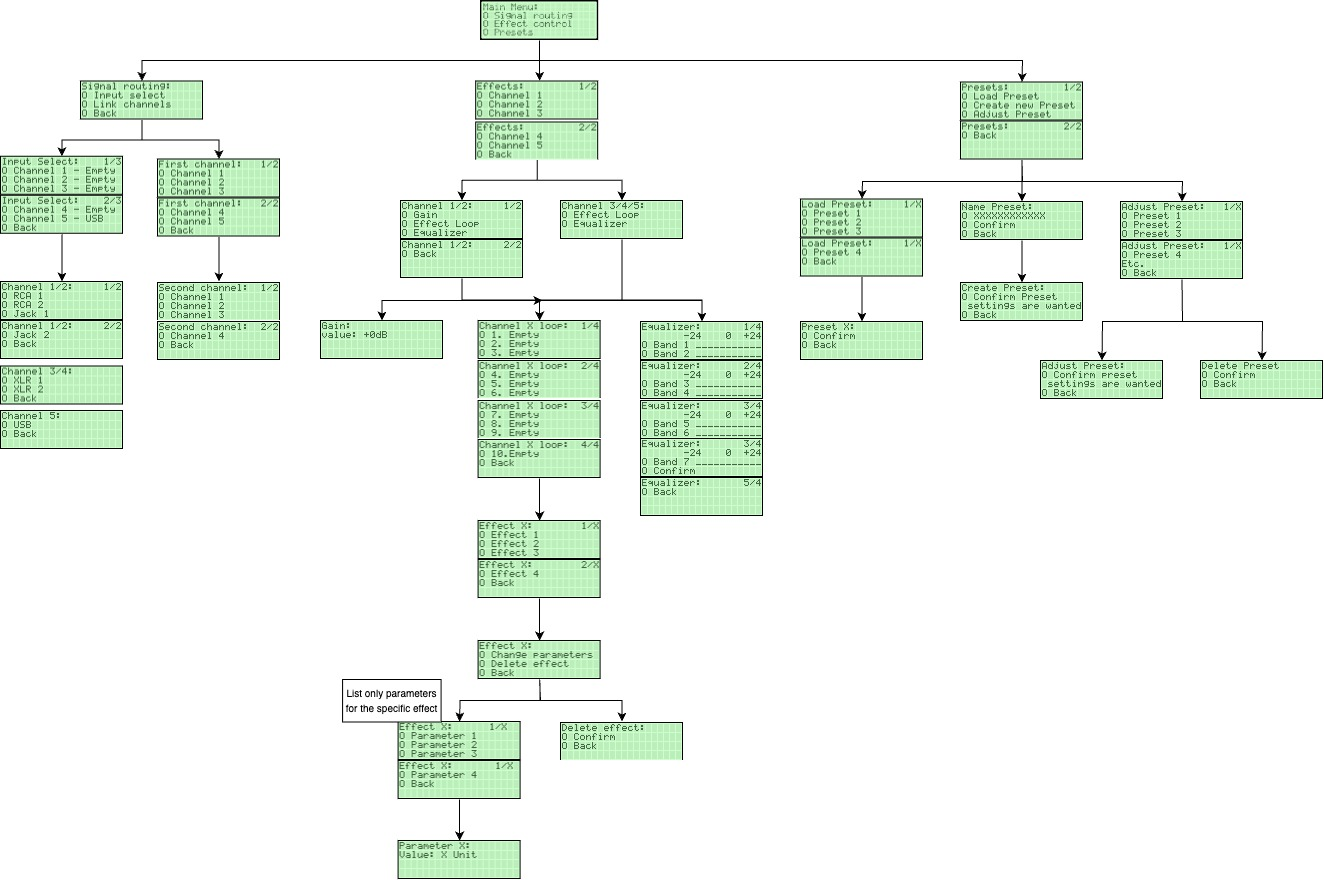
\includegraphics[width=\linewidth]{functionbasedUI}
    \caption{Function Based UI Design for a liquidCrystal screen}
    \label{fig:functionbasedUI}
\end{figure}

This UI is easy to understand when first using the DSP. Options and settings are easy to find from the first menu screen. While a channel based UI is unclear because every option is branched off from the channel select.

\section{Nextion screen}

For this project a Nextion screen is used. This screen can easily be programmed. It comes with software which is image based instead of code based. Images can be inserted and "invisible" buttons can be used to make menus out of the inserted images.

This is a neat way to work because now it is possible to create images in Photoshop or a similar application to use for the whole menu design.

    \chapter{Verification}
    \section{Method}
Time has not yet allowed for the creation of a neat and detailed test plan. However, before the voltage regulator boards are soldered onto the main board, they need to be thoroughly tested to verify their functionality. The plan is to create a test table for this purpose, similar to the specification of ICs in datasheets.

\subsection{Hardware}
\subsubsection{Voltage regulators}
For the voltage regulator modules, the following parameters need to be measured to demonstrate proper operation:
-Thorough visual inspection, especially focusing on the soldering process. This includes checking for short circuits, open connections, solder balls, and other defects.
-The converter should be powered from a lab power supply with low current limit settings. In case of a short circuit or other module defect, the dissipated power will be limited, allowing for the identification and resolution of the issue.
-The output voltage of the converter should be observed using an oscilloscope. Attention should be paid to the absolute accuracy and the amplitude of the ripple voltage.
-The temperature of the PCBA should be monitored to ensure that the module does not get too hot, which could potentially shorten its lifespan.

\subsubsection{Main board}
The functionality of the main board should be verified in the following manner:
-Perform a thorough visual inspection, with a focus on the soldering process. Check for short circuits, open connections, solder balls, and other defects.
-Power the main board from a lab power supply with low current limit settings. This will limit the dissipated power in case of a short circuit or module defect, enabling identification and resolution of the issue. A thermal camera can be used to inspect the PCBA for hotspots.
-Verify the presence and correctness of all power rails.
-Verify that the output of the GPIO pins corresponds to the desired outcome.(e.g. check the SLCK).
-Next, apply a known signal (e.g., a 1kHz sinusoidal waveform with an amplitude of 100mV) to the various inputs of the audio-DSP. If no filters are selected and the audio-DSP is essentially in a pass-through state, the same signal should appear on the selected outputs. The accuracy of this signal can be verified using an audio analyzer such as the AP SYS 2700.

\subsection{Firmware}
The firmware can be tested by simulating the VHDL code in Modelsim. For this .do files are made to force input signals. Due to time constrains only the I2S decoder and encoder have been tested with real audio. 

\subsubsection{I2S decoder and encoder}
For testing the I2S decoder and encoder, they are wired in series. So when a random data pattern is going in the decoder the encoder should output the same data pattern.

\subsubsection{I2C master}
The I2C master is tested by simply writing and reading data with the protocol and verifying that the protocol works correctly according to the I2C protocol standards. 

\subsubsection{State-space BPF}
The state-space BPF is tested by inputting a sine wave outputted from a sine wave generator. By using a sine wave as an input it is very easy to expect the outcome. For instance when having the BPF resonance frequency at 1kHz and inputting a 1kHz sine wave, it is expected that the output sine wave has the same amplitude compared to the input sine wave. And when the frequency of the input sine wave does not match that of the BPF resonance frequency, it will be attenuated. 

The best way to check if the band-pass filter works is by changing the frequency of the input sine wave over time to create a kind of frequency spectrum of the band-pass filter response. 

\subsubsection{Effects}
All the effects are tested by inputting a sine wave to the effect and looking at the result. This approach with a simple sine wave input is chosen because with a sine wave input it is very simple to predict the outcome of the effect and then confirm if it works as expected.

\section{Results}

\subsection{Hardware}

\subsubsection{Buck}
Due to the limited time, this verification has not been done yet.

\subsubsection{Linear voltage regulator}
After conducting a thorough visual inspection, it became apparent that a thorough cleaning of the PCBA was necessary. This was because the solder paste used left behind a significant amount of residue. Therefore, the linear voltage regulators were cleaned in an ultrasonic cleaner.

Subsequently, the linear regulators were connected to a lab power supply with current limiting. However, it quickly became evident that the regulators were not functioning properly. After performing several simulations in LTspice, it was suspected that the LEDs, which serve as low-noise voltage references, might have been soldered incorrectly. However, after consulting the datasheet again with several group members, it was confirmed that the LEDs were indeed soldered correctly according to the datasheet.

Since no other plausible causes emerged after further investigation, it was decided to desolder one of the LEDs and measure it out of circuit using a multimeter to determine its polarity and threshold voltage. To the astonishment of the group, it was discovered that the Broadcom datasheet for the HSMH-C170 LED did not match the LEDs actually supplied. The polarity marking in the datasheet was the exact opposite of the actual component. It is unknown whether an incorrect batch was delivered or if the datasheet itself is genuinely incorrect.
%https://nl.mouser.com/datasheet/2/678/AV02_0551EN_DS_HSMx_Cxxx_25Mar2022-1827675.pdf

\subsubsection{Main board}
\paragraph{inspection} Before connecting every module together and placing every component on the main board it is indeed ascertain that the board has flux and solder paste residue together with solder balls that can cause short circuits, therefore the PCBA will be cleaned in the ultrasonic bath, before doing this it is important to know which components are suitable for this. The relays and electrolytic capacitors are not suitable for this, therefore they are soldered after cleaning.  visual inspection has been done on the main board and the power delivery modules. In the second visual inspection there are no signs of shorts and the components are connected properly.
\paragraph{Visual inspection} 

Before connecting every module together and placing every component on the main board it is indeed ascertain that the board has flux and solder paste residue together with solder balls that can cause short circuits, therefore the PCBA will be cleaned in the ultrasonic bath, before doing this it is important to know which components are suitable for this. The relays and electrolytic capacitors are not suitable for this, therefore they are soldered after cleaning.  visual inspection has been done on the main board and the power delivery modules. In the second visual inspection there are no signs of shorts and the components are connected properly.

\paragraph{Vertical riser board}
The vertical riser boards have to be tested before placing it on the main board. These have been tested individually on ripple(not for the linear regulators, no equipment available to measure), output voltage and temperature. See \ref{Appendix-Vertical riser boards} Vertical riser boards in chapter \ref{chap:Appendix-Verification} verification for the outcomes. For the Sepic the output ripple is ~5mV and output is -15.11V which is within specs, the temperature is 70°C at 1A which is feasible but if there is more power required an extra fan can be attached to cool the converter more. The buck converters(see \ref{pdf:5V Buck converter} 5V buck - \ref{pdf:15V Buck converter} 15V buck) in the beginning all had an output of ~1v. This was because the feedback resistors were exchanged together. Therefore they had to be exchanged again and the problem is solved. The output voltage of all the buck converters are within spec. The ripple is ~8-10mV which is also within spec range. The temperature of all the buck converters are below 45°C at 1A. The output of the linear regulators (see \ref{pdf:12V linear regulator-1}12V lin reg up and till \ref{pdf:5V linear regulator-2}5V lin reg) are within specs and the temperature is 80°C at 1A, they won't be conducting more current than that so the temp is within spec range.

\paragraph{Main board power}
The PCBA is inspected and no short circuit is detected. The next step is to check all the power modules within the PCBA with current limiting, so that the board will not be catch on fire if there is somehow still a short. This has been done with a power supply limited to 1A. All the power rails are tested and every power delivery module is working properly at the desired voltage. The 12V buck converter that is going to the FPGA is tested separately first with four 33 resistors connected in parallel which will give 1.5A of current at 12V. The buck is still below 50°C. Therefore it is safe to power the fpga with the 12V buck converter

\paragraph{FPGA GPIO}
After doing visual inspection and vertical riser board inspection, it is safe to connect the fpga with the main board using flat cables. Unfortunately after connecting the the main board with the fpga it is stated that it didn't work after connecting the laptop using an RCA-cable to the audio dsp. The first thing that has been checked is the output of the clock going to the mainboard from the fpga. Doing so it has been identified that indeed the clock was not being transmitted correctly via the gpio pins of the DE1-SOC. In figure \ref{fig:Appendix-24.576MHz clock output} 24.576MHz clock output it is clearly visible that the 24.567MHz signal is clearly filtered due to parasitic capacitances in the signal path. Those effecting the paths are the following components Mosfets, diodes and the 47 ohm resistor at the GPIO pins. In figure \ref{fig:Appendix-50MHz clock output} 50MHz clock output is visible that the signal is even more weakened which makes it evident it is due to parasitic capacitances. In figure \ref{fig:Appendix-1MHz clock output} 1MHz clock output it is visible that the rising edge of the clock is already behaving capacitive. To be sure that the underlying issue is on all boards and not specifically on this board we have tested the clock output on another board and unfortunately the outcome is the same.

\subsection{Firmware}
\subsubsection{I2S encoder and decoder}
The results of this test can be found in figure \ref{fig:sim_result_i2s_dec_enc}. These results show that the I2S encoder and decoder work as expected. 

\subsubsection{I2C master}
The results can be seen in figure \ref{fig:sim_result_i2c-master}. In this result it can be seen that the I2C master works as expected according to the protocol standards.

\subsubsection{State-space BPF}
For testing the state-space BPF it is very easy to see if it works by checking the frequency response. For the test a resonance frequency for BPF of 400Hz is chosen. Then the sine wave changes its frequency every 10ms. The frequency start at 25Hz and steps up in octaves. The end frequency is 51200Hz as this is far beyond the range of the sampling frequency. The result of this test is seen in \nameref{chap:appendix-G-simulation-results}. 

As expected, the amplitude of the sine wave at the matching resonance frequency of 400Hz is equal to the input amplitude. And when the frequency goes an octave lesser or higher in frequency the amplitude is $\frac{\sqrt{2}}{2}$ times the input amplitude (-3dB). This is a result that is expected from a BPF, therefore it is shown that the BPF works in simulation.

\subsubsection{Effects}
\paragraph{Volume control}


\section{Conclusions}
\subsection{Hardware}

\subsubsection{Buck}
Due to the limited time, this verification has not been done yet.

\subsubsection{SEPIC}
The SEPIC appears to be functioning well after some quick measurements. With an input voltage of +12V, it generates a stable -15V output voltage, and the voltage ripple remains nearly constant regardless of the output current. This aligns with the calculations and simulations. Additionally, the amplitude of the output ripple voltage closely matches the calculated and simulated values.

\subsubsection{Linear voltage regulator}
Due to the limited time, this verification has not yet been completed.

\subsubsection{Main board}
Due to the limited time, this verification has not been done yet.

\subsection{Firmware}
The I2S decoder, I2S encoder and I2C master work as expected. Therefore it is possible to sample audio using the ADC and DAC of the FPGA board. This has been tested and verified that this works. 

Due to time constrains further testing and implementation of the effects has not been conducted. 


    \chapter{Conclusions}
    Due to time constrains the final project is not yet working. The hardware main board has been tested for as far as possible and works for as far as could be tested. Also all the vertical riser boards have been tested and validated as shown in the verification chapter. The firmware that has been developed for the product has been tested in ModelSim and works there, but still has to be implemented in combination with the hardware. 
\par
<<<<<<< HEAD
\noindent During testing of the DE1-SOC board a problem has been found. The clock signal that goes from the FPGA to the DAC's and ADC's is not working properly. The output of the DE1-SOC FPGA board seems to be to capacitive due to parasitics of the board design and therefore the clock signal gets filtered down and is not picked up by the ADC's and DAC's. The schematic of the FPGA board shows that there is a 47 Ω series resistor, this in combination with the RDS(on) of the internal switching FETs of the Cyclone-V and the capacitance of the TVS diode in parallel with the parasitic capacitance of the PCB seems to cause the clock signal to be filtered out as an Rc-LPF. The measurements where done on the DE1-SOC board that was not connected to the Main board of the DSP to exclude our main board and flat cable from this conclusion.
=======
\noindent During testing of the DE1-SOC board a problem has been found. The clock signal that goes from the FPGA to the DACs and ADCs is not working properly. The output of the DE1-SOC FPGA board seems to be to capacitive due to parasitics of the board design and therefore the clock signal gets filtered down and is not picked up by the ADCs and DACs. The schematic of the FPGA board shows that there is a 47 Ohm series resistor, this in combination with the RDS(on) of the internal switching FETs of the Cyclone-V and the capacitance of the TVS diode in parallel with the parasitic capacitance of the PCB seems to cause the clock signal to be filtered out as an RC-LPF. The measurements where done on the DE1-SOC board that was not connected to the Main board of the DSP to exclude our main board and flat cable from this conclusion.
>>>>>>> 6baa9264baaf424ca591278f70fbd15759b66a8a


    \chapter{Recommendations}
    Due to time constraints the project has not yet been finished. Most parts have been tested and work as expected, but some parts still have to be implemented and tested according to the planning. Some more time is needed to finish the Project.
\par
\noindent The following recommendations have been made to help the project work/ work better:

\begin{itemize}
    \setlength\itemsep{-0.3em} %MAKES THE GAP SMALLER BETWEEN 2 ITEMS
    \item Do not use FFT for the processing, use a direct approach instead or use a way more powerful processor
    \item Look into the clock signals from the FPGA board to the main PCB
    \item Investigate if there are other FPGA boards available which do support the needed 24.576 MHz output frequency on their GPIO pins
    \item Indicate on the UI screen which option is selected
    \item Make a less enthusiastic project planning
\end{itemize}

    \chapter*{References}
    \addcontentsline{toc}{chapter}{References}  

    % \chapter*{Appendices}
    % \addcontentsline{toc}{chapter}{Appendices}  
    \addcontentsline{toc}{chapter}{Appendix A: State-space}  
\chapter*{Appendix A: State-space}
\label{chap:appendix-A-statespace}


% \begin{figure}[ht]
    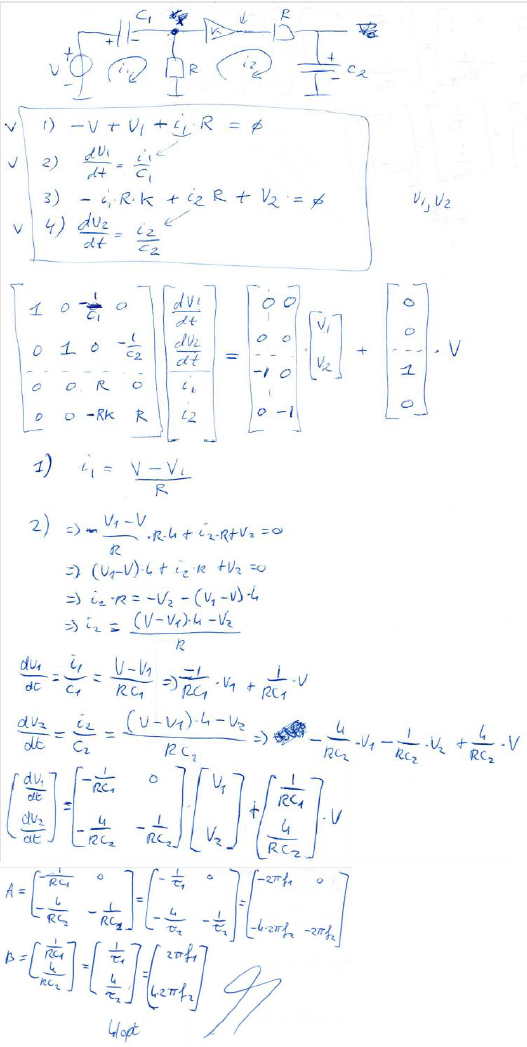
\includegraphics[width=\textwidth, height=0.9\textheight, keepaspectratio]{State-space_notation_solution.png}
%    \caption{State-space notation derived from band-pass filter circuit}
%     \label{fig:state-space-derived-bpf}
% \end{figure}
\newpage
\newpage

\section*{Appendix B: Buck converter schematic}
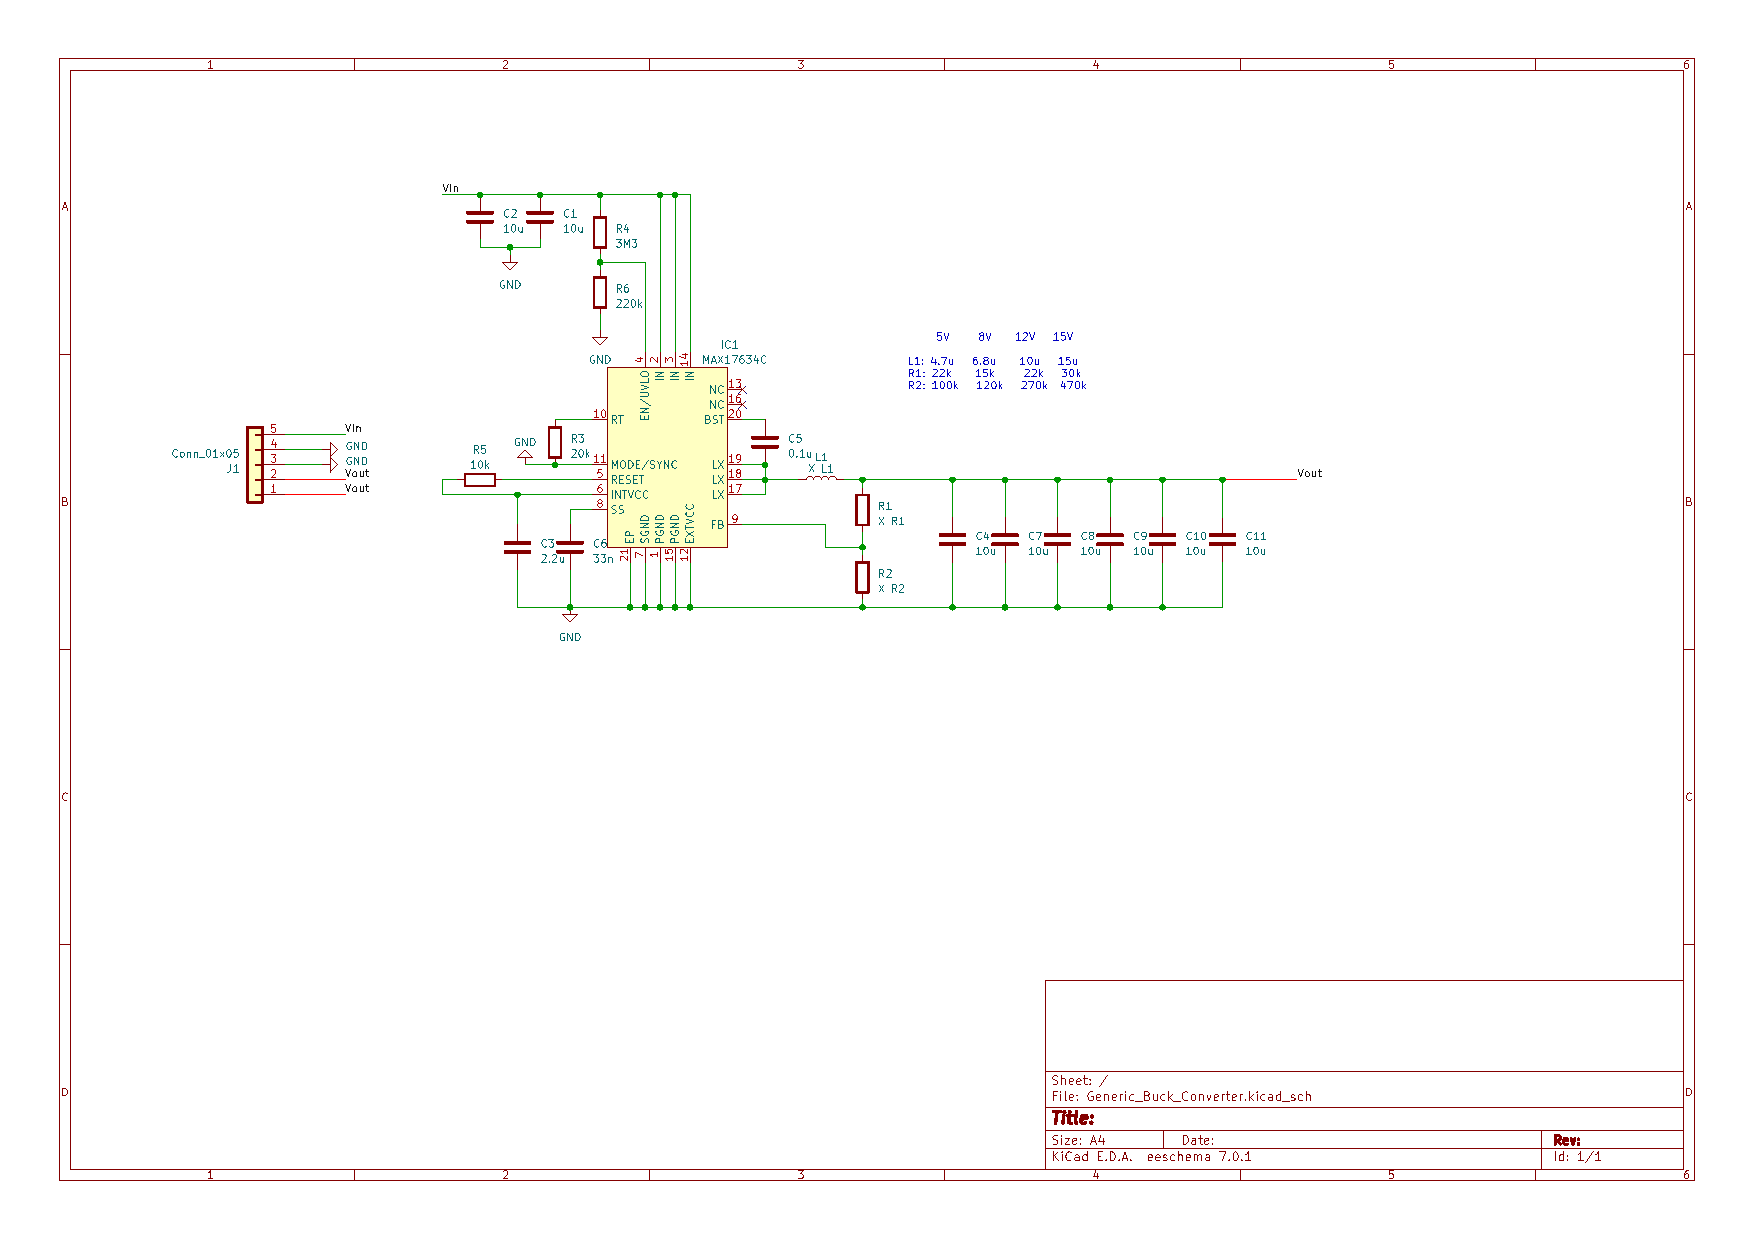
\includegraphics[angle=90, width=500pt]{Generic_Buck_Converter_schematic.pdf}

\section*{Appendix C: SEPIC schematic}
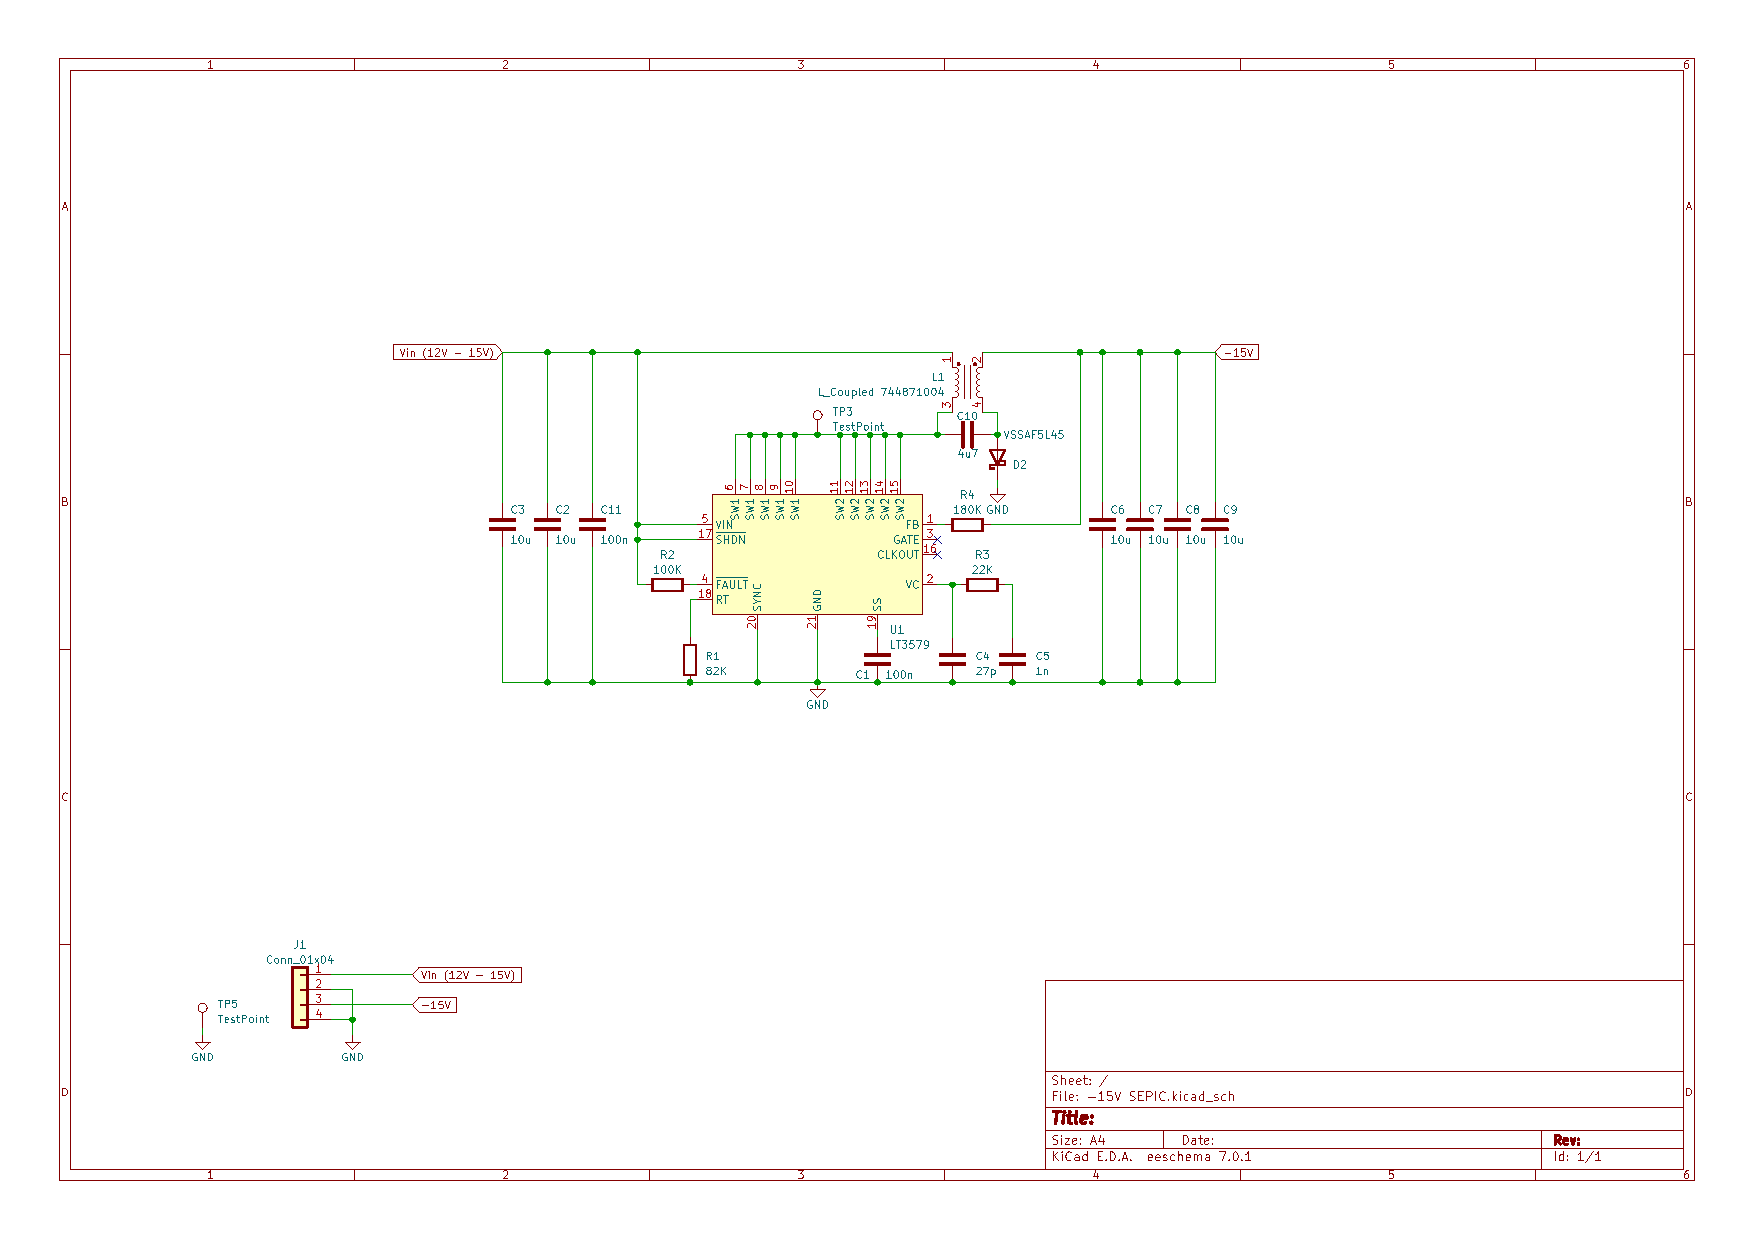
\includegraphics[angle=90, width=500pt]{-15V_SEPIC_schematic.pdf}

\section*{Appendix D: Linear regulator schematic}
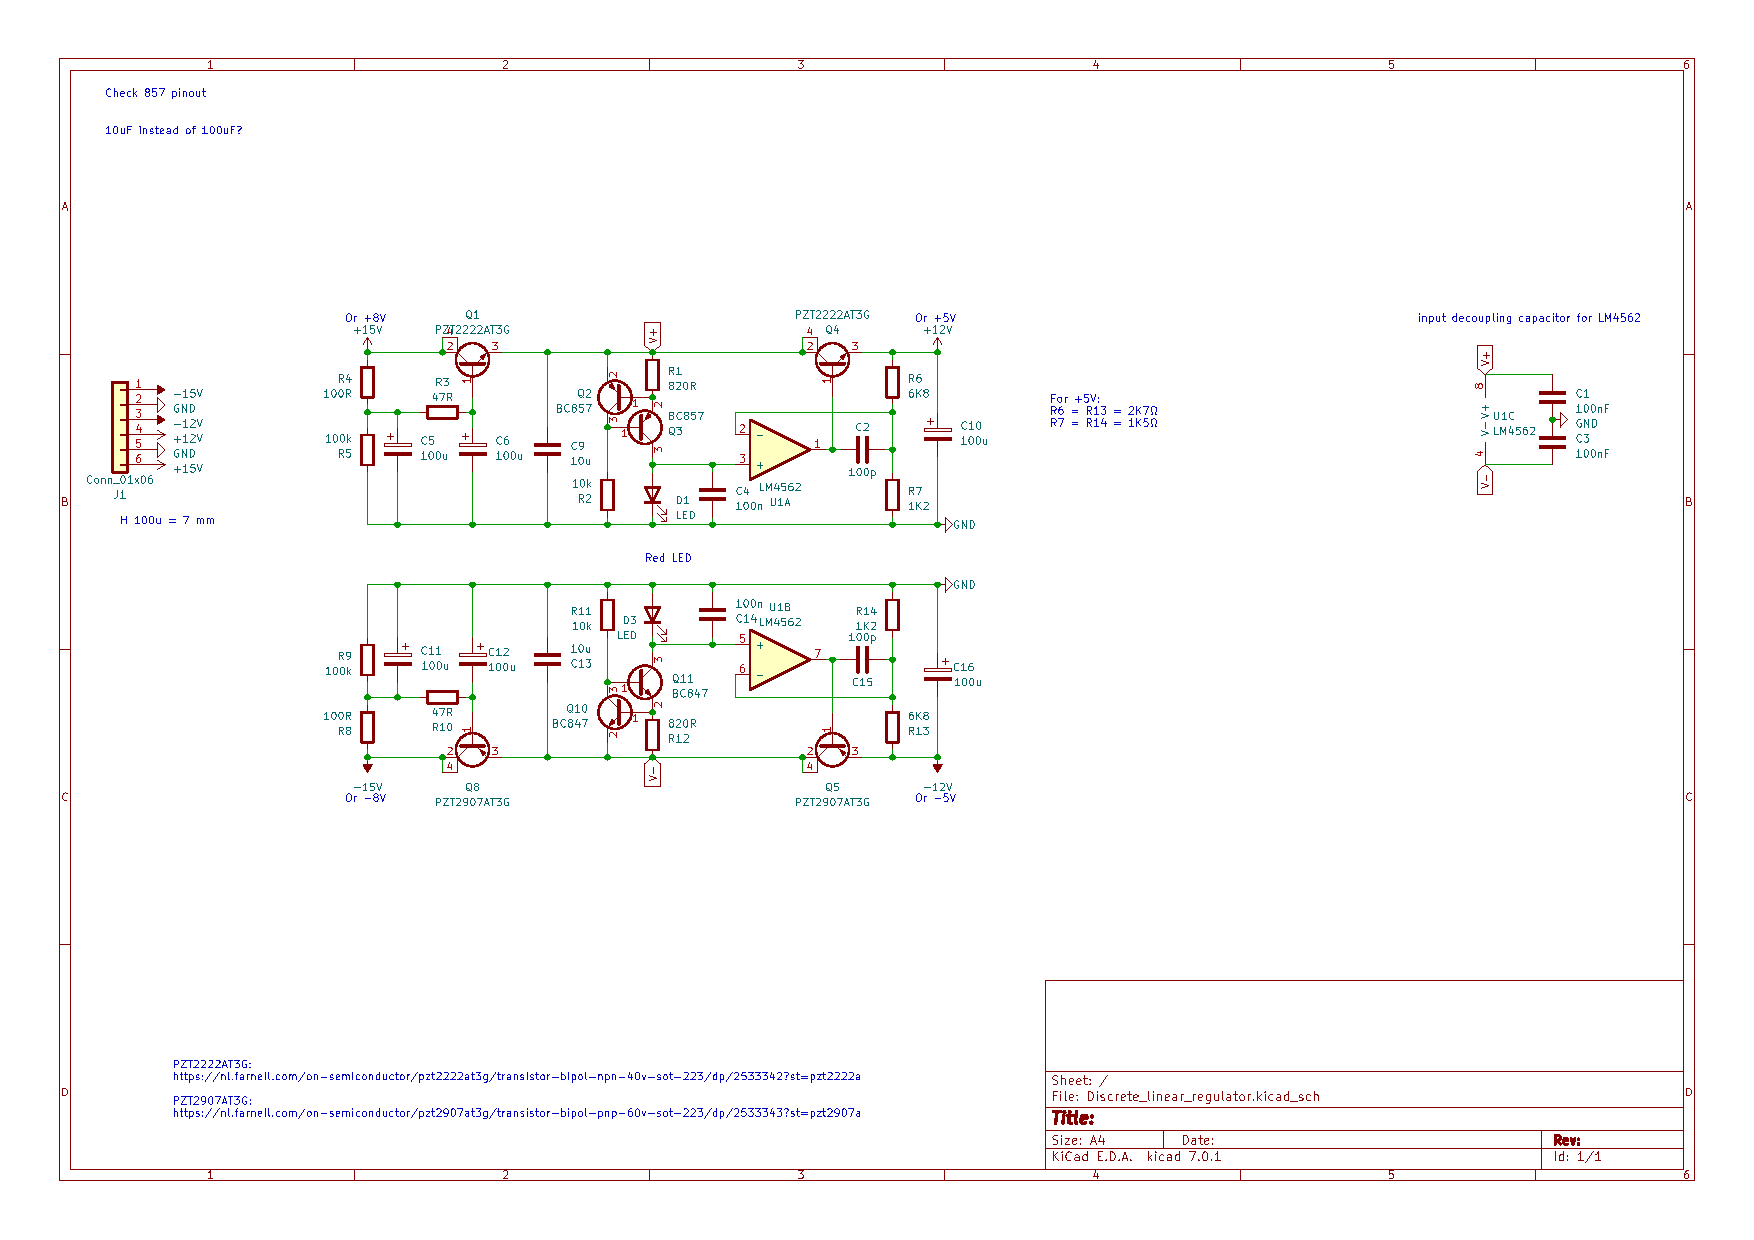
\includegraphics[angle=90, width=500pt]{Discrete_linear_regulator_schematic.pdf}

\section*{Appendix E: Main board schematic}
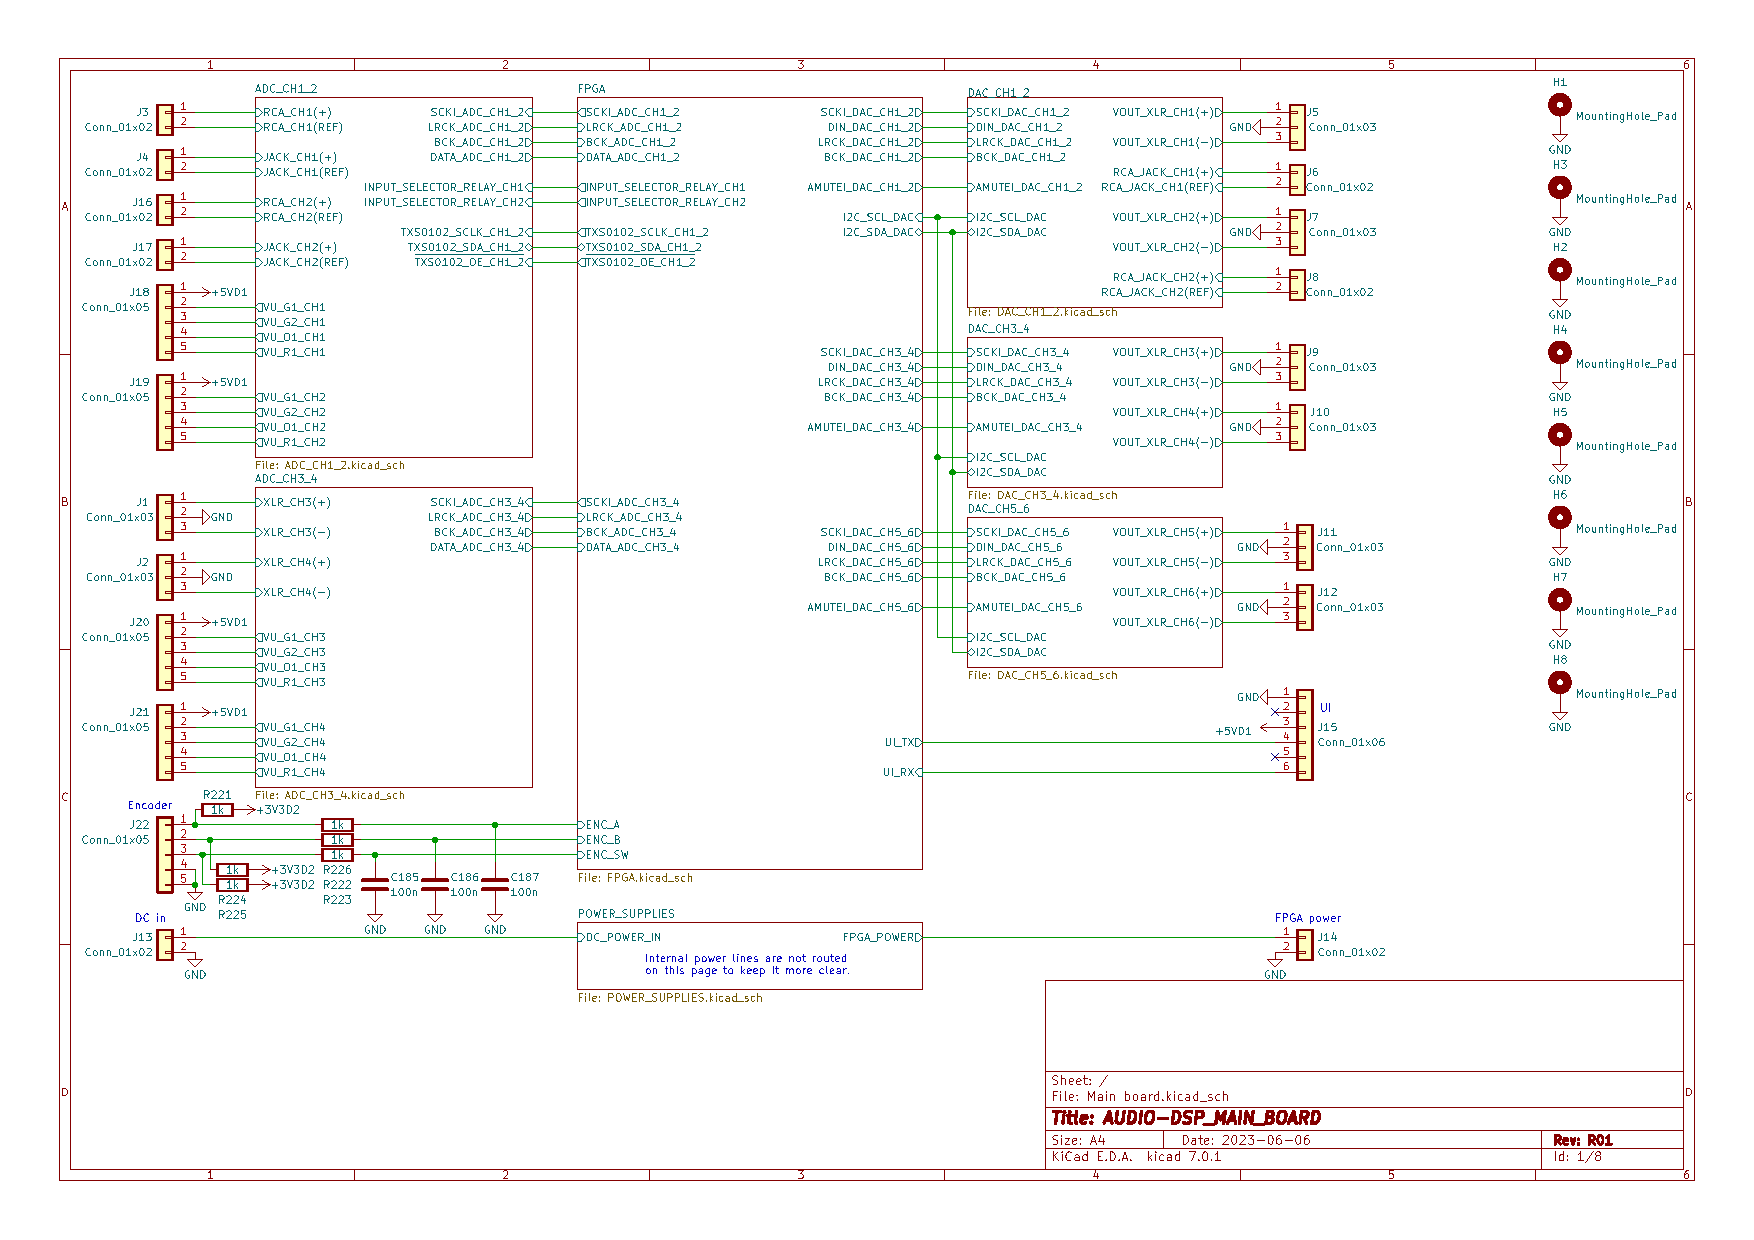
\includepdf[angle=90, pages=-]{Main_board_schematic.pdf}

\section*{Appendix F: UI design} \label{AppendixF}
\begin{figure}[ht]
    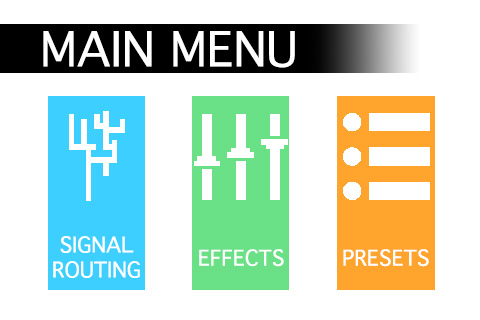
\includegraphics[width=0.7\textwidth]{MainMenu1}
    \caption{Main menu design}
    \label{fig:mainmenu}
\end{figure}

\begin{figure}[ht]
    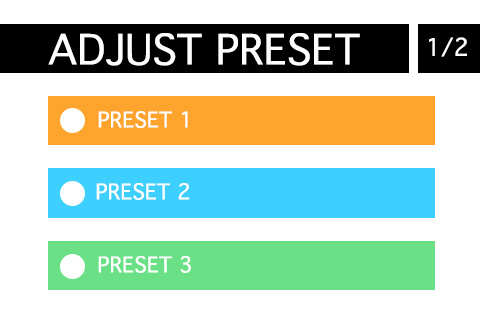
\includegraphics[width=0.7\textwidth]{adjustpreset1-2}
    \caption{Other menu screen, other ones are similar to this one}
    \label{fig:adjustpresetmenu}
\end{figure}

\newpage

\section*{Appendix G: Case} \label{AppendixG}
\begin{figure}[ht]
    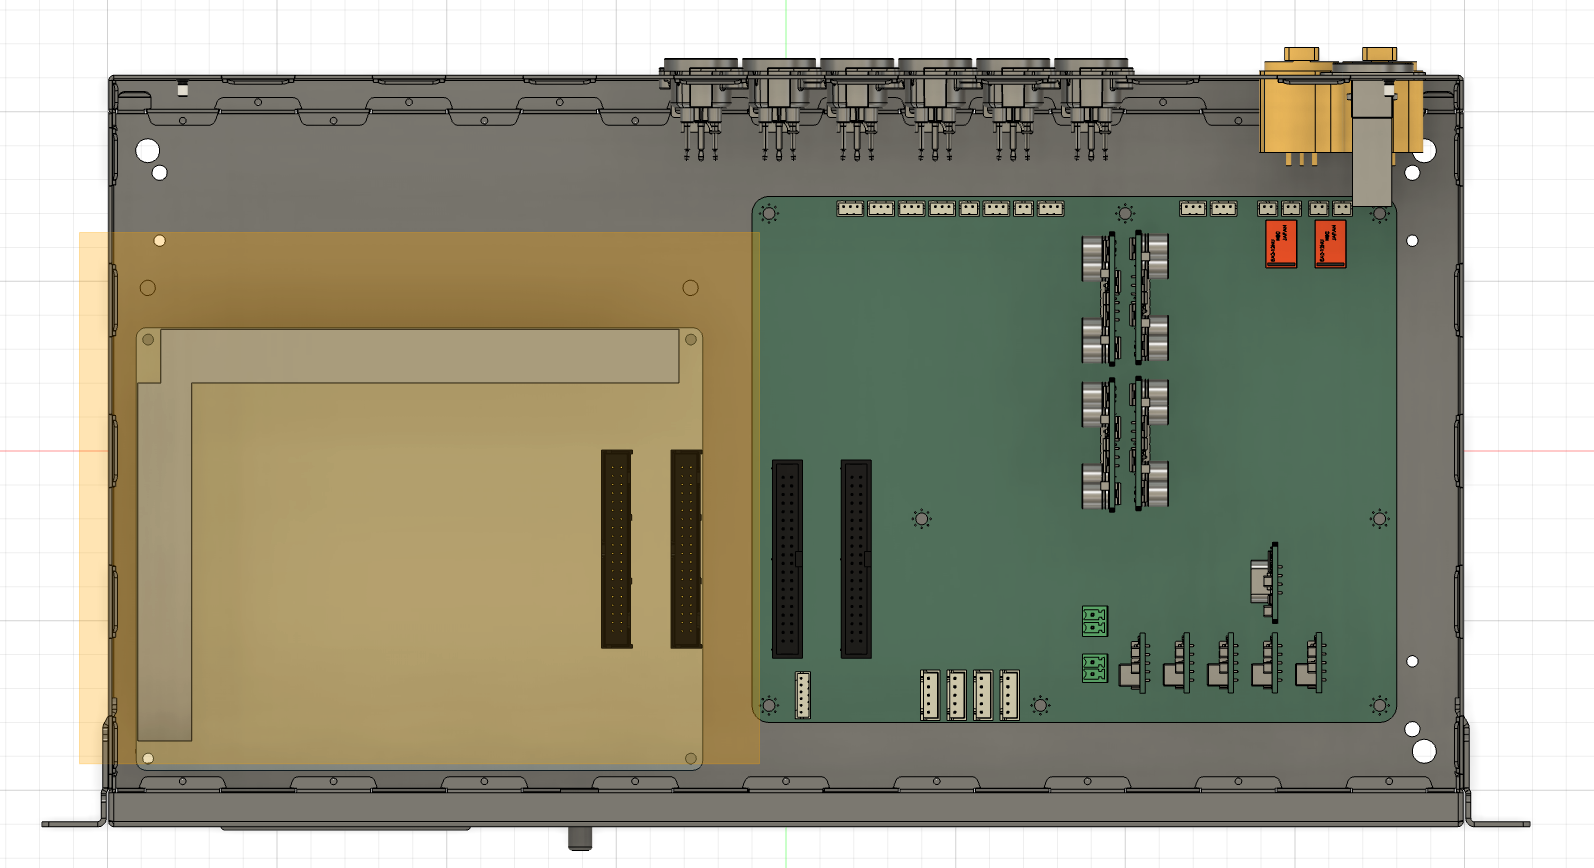
\includegraphics[width=0.8\textwidth]{topviewcase}
    \caption{Top-down view of the case}
    \label{fig:topview}
\end{figure}

\begin{figure}[ht]
    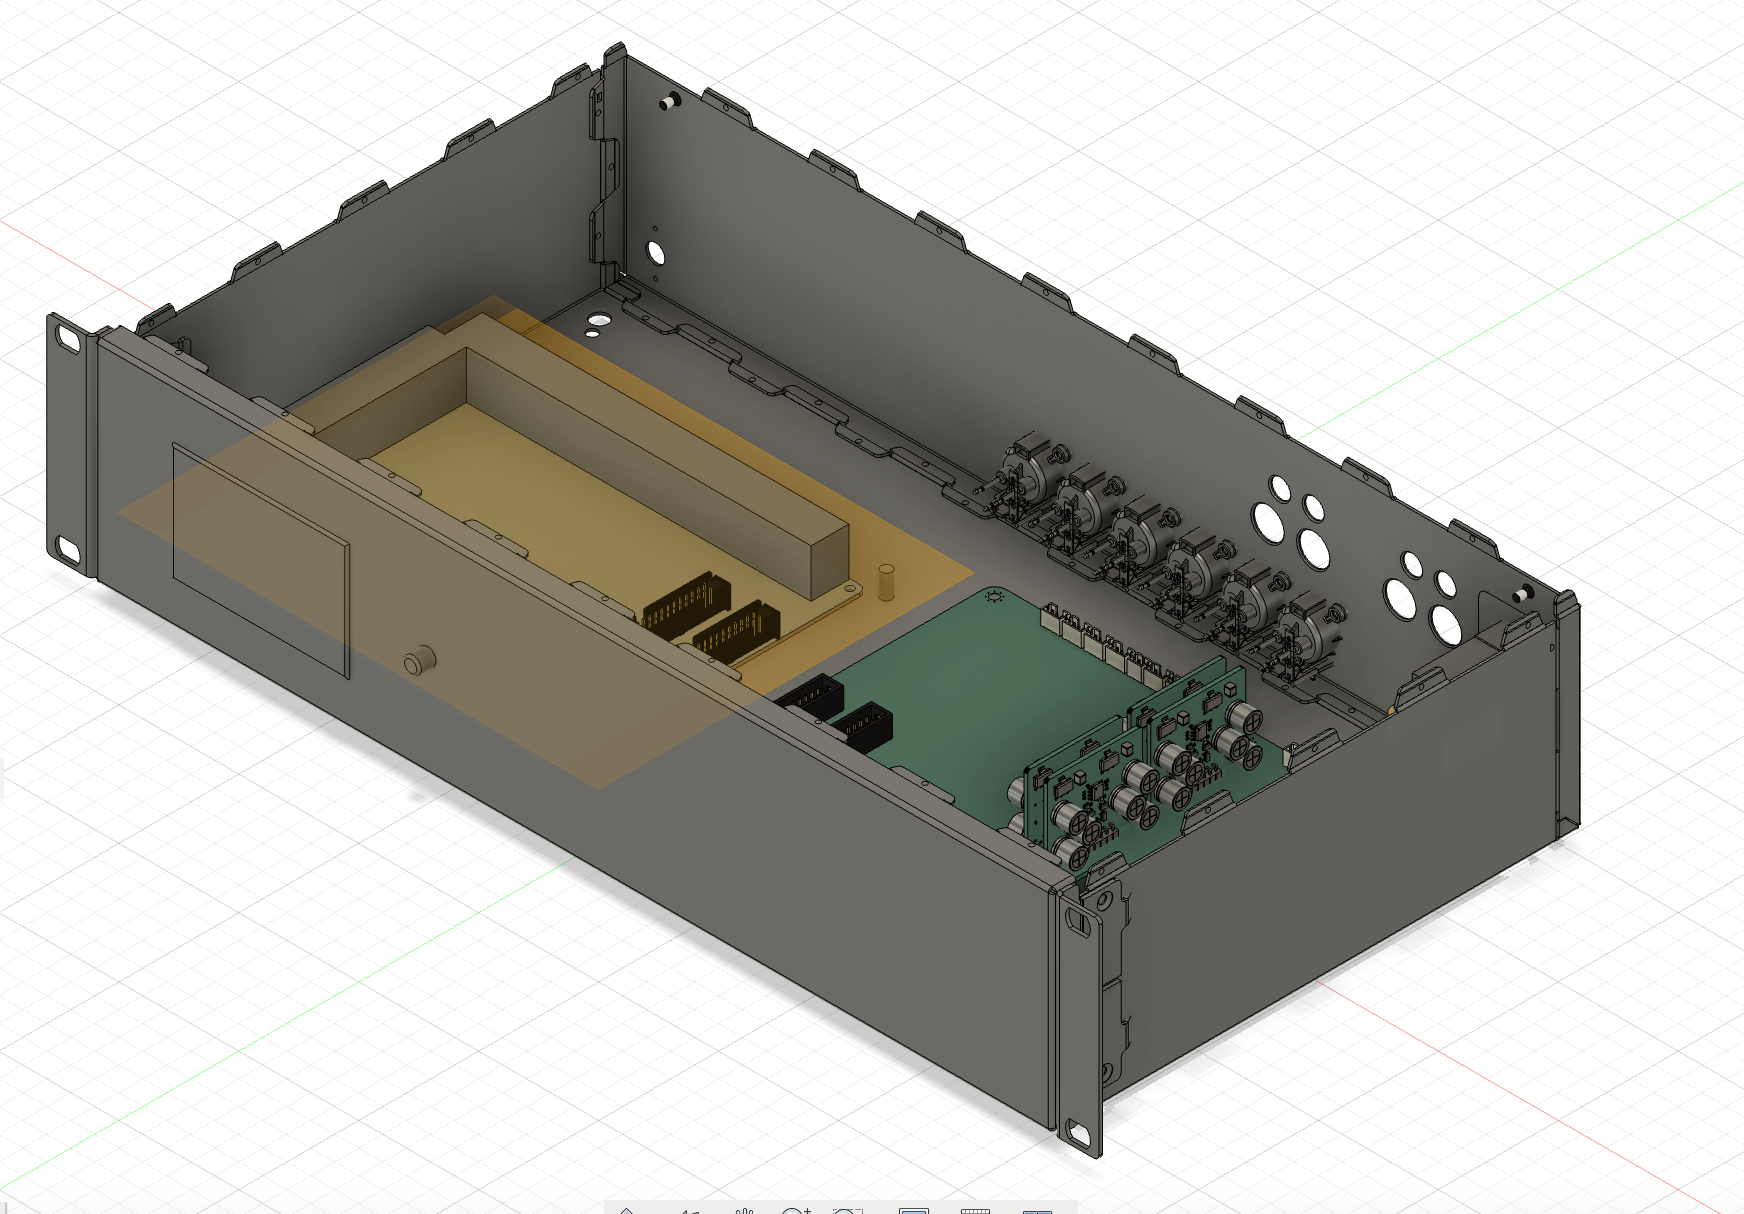
\includegraphics[width=0.8\textwidth]{frontviewcase}
    \caption{Front view of the case}
    \label{fig:frontview}
\end{figure}

\begin{figure}[ht]
    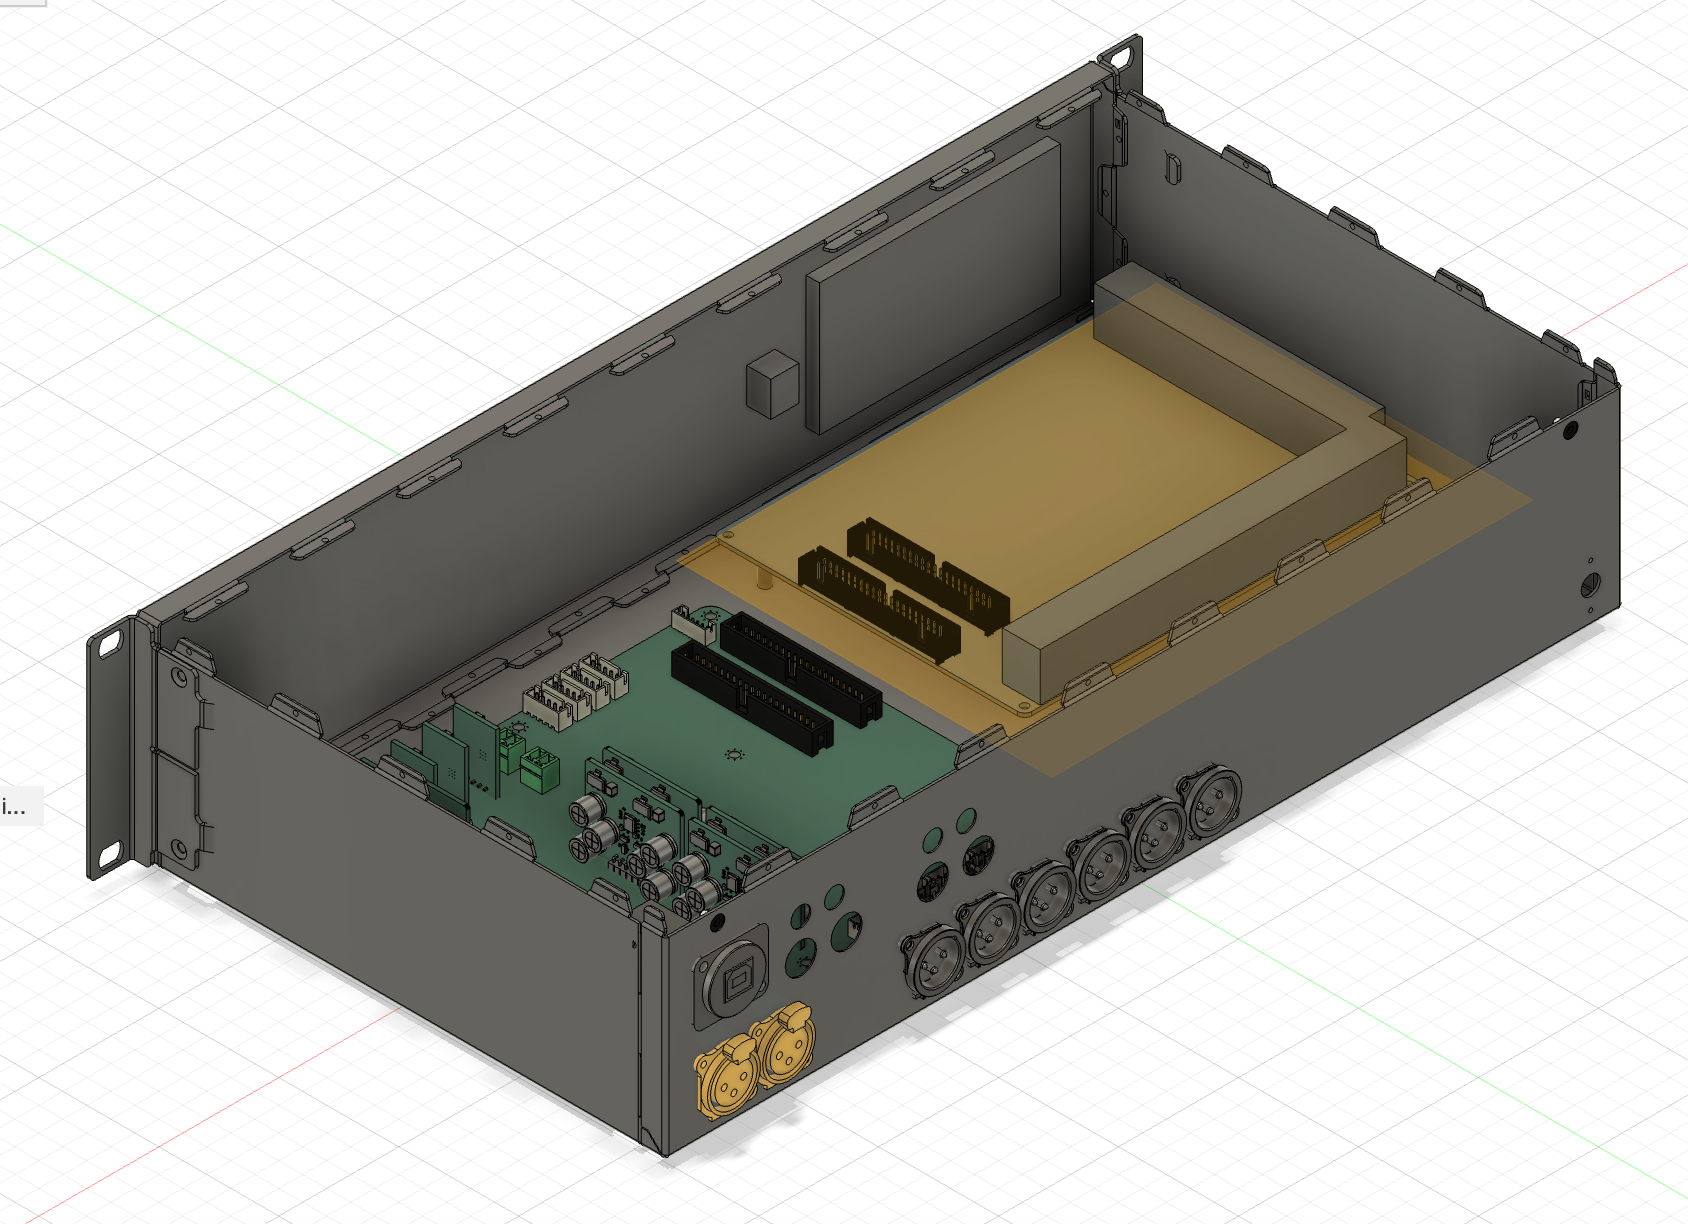
\includegraphics[width=0.8\textwidth]{rearviewcase}
    \caption{Rear view of the case}
    \label{fig:rearview}
\end{figure}

\newpage


    \addcontentsline{toc}{chapter}{Appendix B: VHDL code}  
\chapter*{Appendix B: VHDL code}
\label{chap:appendix-B-vhdl}

\section*{I2S Decoder}
\addcontentsline{toc}{section}{I2S Decoder}
\begin{lstlisting}
LIBRARY IEEE;
USE IEEE.STD_LOGIC_1164.ALL;
USE IEEE.NUMERIC_STD.ALL;

ENTITY i2s_decoder IS
	GENERIC (
	d_width : INTEGER := 24); --data width
	PORT (
		nrst : IN std_logic; --active-low reset
		sck : IN std_logic; --serial clock
		ws : IN std_logic; --left right audio word select
		sd : IN std_logic; --serial data
		data_left : OUT std_logic_vector(d_width - 1 DOWNTO 0); --left audio data
		data_right : OUT std_logic_vector(d_width - 1 DOWNTO 0); --right audio data
		o_avail_left : OUT std_logic; --left audio available
		o_avail_right : OUT std_logic --right audio available
	); 
END i2s_decoder;

ARCHITECTURE Behavioral OF i2s_decoder IS
	SIGNAL l_data_int : std_logic_vector(d_width - 1 DOWNTO 0); --internal left audio data
	SIGNAL r_data_int : std_logic_vector(d_width - 1 DOWNTO 0); --internal right audio data

	TYPE t_machine IS (ready, rd_l, rd_r);
	SIGNAL machine : t_machine := ready; --state machine

	SIGNAL bit_cnt : INTEGER := 0; --bit counter

BEGIN
	PROCESS (sck, nrst)
	BEGIN
		IF nrst = '0' THEN
			--Reset state machine and bit counter
			machine <= ready;
			bit_cnt <= 0;
		ELSIF rising_edge(sck) THEN
			CASE machine IS
				--Read left audio
				WHEN rd_l => 
					--Have all bits been read
					IF bit_cnt < d_width THEN
						bit_cnt <= bit_cnt + 1; --increment bit counter
						l_data_int <= l_data_int(l_data_int'HIGH - 1 DOWNTO 0) & sd; --shift serial data in internal left audio data
						data_right <= r_data_int; --output right audio data
					END IF;

					--Write available bits
					o_avail_left <= '0';
					o_avail_right <= '1';
					--Read right audio
				WHEN rd_r => 
					--Have all bits been read
					IF bit_cnt < d_width THEN
						bit_cnt <= bit_cnt + 1; --increment bit counter
						r_data_int <= r_data_int(r_data_int'HIGH - 1 DOWNTO 0) & sd; --shift serial data in internal right audio data
						data_left <= l_data_int; --output left audio data
					END IF;

					--Write available bits
					o_avail_left <= '1';
					o_avail_right <= '0';
				WHEN OTHERS => 
					NULL;
			END CASE;

			--Left audio data is selected and not already reading left audio data
			IF ws = '0' AND machine /= rd_l THEN
				bit_cnt <= 0; --reset bit counter 
				machine <= rd_l; --set state to read left channel
				--Right audio data is selected and not already reading right audio data
			ELSIF ws = '1' AND machine /= rd_r THEN
				bit_cnt <= 0; --reset bit counter
				machine <= rd_r; --set state to read right channel
			END IF;
		END IF;
	END PROCESS;

END Behavioral;
\end{lstlisting}

\section*{I2S Encoder}
\addcontentsline{toc}{section}{I2S Encoder}
\begin{lstlisting}
LIBRARY IEEE;
USE IEEE.STD_LOGIC_1164.ALL;
USE IEEE.NUMERIC_STD.ALL;

ENTITY i2s_encoder IS
	GENERIC (
	d_width : INTEGER := 24); --data width
	PORT (
		nrst : IN std_logic; --active-low reset
		sck : IN std_logic; --serial clock
		ws : IN std_logic; --left right audio word select
		data_left : IN std_logic_vector(d_width - 1 DOWNTO 0); --left audio data
		data_right : IN std_logic_vector(d_width - 1 DOWNTO 0); --right audio data
		sd : OUT std_logic; --serial data
		i_avail_left : IN std_logic; --left audio available
		i_avail_right : IN std_logic --right audio available
	); 
END i2s_encoder;

ARCHITECTURE Behavioral OF i2s_encoder IS
	SIGNAL l_data_int : std_logic_vector(d_width - 1 DOWNTO 0); --internal left audio data
	SIGNAL r_data_int : std_logic_vector(d_width - 1 DOWNTO 0); --internal right audio data

	TYPE t_machine IS (ready, wr_l, wr_r);
	SIGNAL machine : t_machine := ready; --state machine

	SIGNAL bit_cnt : INTEGER := 0; --bit counter

BEGIN
	PROCESS (sck, nrst)
	BEGIN
		IF nrst = '0' THEN
			--Reset state machine and bit counter
			machine <= ready;
			bit_cnt <= 0;
		ELSIF falling_edge(sck) THEN
			CASE machine IS
				--Write left audio
				WHEN wr_l => 
					--Have all bits been written
					IF bit_cnt < d_width THEN
						bit_cnt <= bit_cnt + 1; --increment bit counter
						l_data_int <= l_data_int(r_data_int'HIGH - 1 DOWNTO 0) & '0'; --shift internal left audio data to the left
						sd <= l_data_int(l_data_int'high); --output MSB of internal left audio data to serial data output
					END IF;

					--If right data is available
					IF (i_avail_right = '1') THEN
						r_data_int <= data_right;
					END IF;

					--Write right audio
				WHEN wr_r => 
					--Have all bits been written
					IF bit_cnt < d_width THEN
						bit_cnt <= bit_cnt + 1; --increment bit counter
						r_data_int <= r_data_int(r_data_int'HIGH - 1 DOWNTO 0) & '0'; --shift internal right audio data to the left
						sd <= r_data_int(r_data_int'high); --output MSB of internal right audio data to serial data output
					END IF;

					--If left data is available
					IF (i_avail_left = '1') THEN
						l_data_int <= data_left;
					END IF;

				WHEN OTHERS => 
					NULL;
			END CASE;
 
			--Left audio data is selected and not already writing left audio data
			IF ws = '0' AND machine /= wr_l THEN
				bit_cnt <= 0; --reset bit counter
				machine <= wr_l; --set state to write left channel
				--Right audio data is selected and not already writing right audio data
			ELSIF ws = '1' AND machine /= wr_r THEN
				bit_cnt <= 0; --reset bit counter
				machine <= wr_r; --set state to write right channel
			END IF;
		END IF;
	END PROCESS;
END Behavioral;
\end{lstlisting}

\section*{I2C master code}
\addcontentsline{toc}{section}{I2C master code}
\begin{lstlisting}
LIBRARY ieee;
USE ieee.std_logic_1164.ALL;
USE ieee.std_logic_unsigned.ALL;

ENTITY i2c_master IS
    GENERIC (
        input_clk : INTEGER := 50_000_000; --input clock speed from user logic in Hz
    bus_clk : INTEGER := 400_000); --speed the i2c bus (scl) will run at in Hz
    PORT (
        clk : IN STD_LOGIC; --system clock
        reset_n : IN STD_LOGIC; --active low reset
        ena : IN STD_LOGIC; --latch in command
        addr : IN STD_LOGIC_VECTOR(6 DOWNTO 0); --address of target slave
        rw : IN STD_LOGIC; --'0' is write, '1' is read
        data_wr : IN STD_LOGIC_VECTOR(7 DOWNTO 0); --data to write to slave
        busy : OUT STD_LOGIC; --indicates transaction in progress
        data_rd : OUT STD_LOGIC_VECTOR(7 DOWNTO 0); --data read from slave
        ack_error : BUFFER STD_LOGIC; --flag if improper acknowledge from slave
        sda : INOUT STD_LOGIC; --serial data output of i2c bus
    scl : INOUT STD_LOGIC); --serial clock output of i2c bus
END i2c_master;

ARCHITECTURE logic OF i2c_master IS
    CONSTANT divider : INTEGER := (input_clk/bus_clk)/4; --number of clocks in 1/4 cycle of scl
    TYPE machine IS(ready, start, command, slv_ack1, wr, rd, slv_ack2, mstr_ack, stop); --needed states
    SIGNAL state : machine; --state machine
    SIGNAL data_clk : STD_LOGIC; --data clock for sda
    SIGNAL data_clk_prev : STD_LOGIC; --data clock during previous system clock
    SIGNAL scl_clk : STD_LOGIC; --constantly running internal scl
    SIGNAL scl_ena : STD_LOGIC := '0'; --enables internal scl to output
    SIGNAL sda_int : STD_LOGIC := '1'; --internal sda
    SIGNAL sda_ena_n : STD_LOGIC; --enables internal sda to output
    SIGNAL addr_rw : STD_LOGIC_VECTOR(7 DOWNTO 0); --latched in address and read/write
    SIGNAL data_tx : STD_LOGIC_VECTOR(7 DOWNTO 0); --latched in data to write to slave
    SIGNAL data_rx : STD_LOGIC_VECTOR(7 DOWNTO 0); --data received from slave
    SIGNAL bit_cnt : INTEGER RANGE 0 TO 7 := 7; --tracks bit number in transaction
    SIGNAL stretch : STD_LOGIC := '0'; --identifies if slave is stretching scl
BEGIN
    --generate the timing for the bus clock (scl_clk) and the data clock (data_clk)
    PROCESS (clk, reset_n)
    VARIABLE count : INTEGER RANGE 0 TO divider * 4; --timing for clock generation
    BEGIN
        IF (reset_n = '0') THEN --reset asserted
            stretch <= '0';
            count := 0;
        ELSIF (clk'EVENT AND clk = '1') THEN
            data_clk_prev <= data_clk; --store previous value of data clock
            IF (count = divider * 4 - 1) THEN --end of timing cycle
                count := 0; --reset timer
            ELSIF (stretch = '0') THEN --clock stretching from slave not detected
                count := count + 1; --continue clock generation timing
            END IF;
            CASE count IS
                WHEN 0 TO divider - 1 => --first 1/4 cycle of clocking
                    scl_clk <= '0';
                    data_clk <= '0';
                WHEN divider TO divider * 2 - 1 => --second 1/4 cycle of clocking
                    scl_clk <= '0';
                    data_clk <= '1';
                WHEN divider * 2 TO divider * 3 - 1 => --third 1/4 cycle of clocking
                    scl_clk <= '1'; --release scl
                    IF (scl = '0') THEN --detect if slave is stretching clock
                        stretch <= '1';
                    ELSE
                        stretch <= '0';
                    END IF;
                    data_clk <= '1';
                WHEN OTHERS => --last 1/4 cycle of clocking
                    scl_clk <= '1';
                    data_clk <= '0';
            END CASE;
        END IF;
    END PROCESS;

    --state machine and writing to sda during scl low (data_clk rising edge)
    PROCESS (clk, reset_n)
        BEGIN
            IF (reset_n = '0') THEN --reset asserted
                state <= ready; --return to initial state
                busy <= '1'; --indicate not available
                scl_ena <= '0'; --sets scl high impedance
                sda_int <= '1'; --sets sda high impedance
                ack_error <= '0'; --clear acknowledge error flag
                bit_cnt <= 7; --restarts data bit counter
                data_rd <= "00000000"; --clear data read port
            ELSIF (clk'EVENT AND clk = '1') THEN
                IF (data_clk = '1' AND data_clk_prev = '0') THEN --data clock rising edge
                    CASE state IS
                        WHEN ready => --idle state
                            IF (ena = '1') THEN --transaction requested
                                busy <= '1'; --flag busy
                                addr_rw <= addr & rw; --collect requested slave address and command
                                data_tx <= data_wr; --collect requested data to write
                                state <= start; --go to start bit
                            ELSE --remain idle
                                busy <= '0'; --unflag busy
                                state <= ready; --remain idle
                            END IF;
                        WHEN start => --start bit of transaction
                            busy <= '1'; --resume busy if continuous mode
                            sda_int <= addr_rw(bit_cnt); --set first address bit to bus
                            state <= command; --go to command
                        WHEN command => --address and command byte of transaction
                            IF (bit_cnt = 0) THEN --command transmit finished
                                sda_int <= '1'; --release sda for slave acknowledge
                                bit_cnt <= 7; --reset bit counter for "byte" states
                                state <= slv_ack1; --go to slave acknowledge (command)
                            ELSE --next clock cycle of command state
                                bit_cnt <= bit_cnt - 1; --keep track of transaction bits
                                sda_int <= addr_rw(bit_cnt - 1); --write address/command bit to bus
                                state <= command; --continue with command
                            END IF;
                        WHEN slv_ack1 => --slave acknowledge bit (command)
                            IF (addr_rw(0) = '0') THEN --write command
                                sda_int <= data_tx(bit_cnt); --write first bit of data
                                state <= wr; --go to write byte
                            ELSE --read command
                                sda_int <= '1'; --release sda from incoming data
                                state <= rd; --go to read byte
                            END IF;
                        WHEN wr => --write byte of transaction
                            busy <= '1'; --resume busy if continuous mode
                            IF (bit_cnt = 0) THEN --write byte transmit finished
                                sda_int <= '1'; --release sda for slave acknowledge
                                bit_cnt <= 7; --reset bit counter for "byte" states
                                state <= slv_ack2; --go to slave acknowledge (write)
                            ELSE --next clock cycle of write state
                                bit_cnt <= bit_cnt - 1; --keep track of transaction bits
                                sda_int <= data_tx(bit_cnt - 1); --write next bit to bus
                                state <= wr; --continue writing
                            END IF;
                        WHEN rd => --read byte of transaction
                            busy <= '1'; --resume busy if continuous mode
                            IF (bit_cnt = 0) THEN --read byte receive finished
                                IF (ena = '1' AND addr_rw = addr & rw) THEN --continuing with another read at same address
                                    sda_int <= '0'; --acknowledge the byte has been received
                                ELSE --stopping or continuing with a write
                                    sda_int <= '1'; --send a no-acknowledge (before stop or repeated start)
                                END IF;
                                bit_cnt <= 7; --reset bit counter for "byte" states
                                data_rd <= data_rx; --output received data
                                state <= mstr_ack; --go to master acknowledge
                            ELSE --next clock cycle of read state
                                bit_cnt <= bit_cnt - 1; --keep track of transaction bits
                                state <= rd; --continue reading
                            END IF;
                        WHEN slv_ack2 => --slave acknowledge bit (write)
                            IF (ena = '1') THEN --continue transaction
                                busy <= '0'; --continue is accepted
                                addr_rw <= addr & rw; --collect requested slave address and command
                                data_tx <= data_wr; --collect requested data to write
                                IF (addr_rw = addr & rw) THEN --continue transaction with another write
                                    sda_int <= data_wr(bit_cnt); --write first bit of data
                                    state <= wr; --go to write byte
                                ELSE --continue transaction with a read or new slave
                                    state <= start; --go to repeated start
                                END IF;
                            ELSE --complete transaction
                                state <= stop; --go to stop bit
                            END IF;
                        WHEN mstr_ack => --master acknowledge bit after a read
                            IF (ena = '1') THEN --continue transaction
                                busy <= '0'; --continue is accepted and data received is available on bus
                                addr_rw <= addr & rw; --collect requested slave address and command
                                data_tx <= data_wr; --collect requested data to write
                                IF (addr_rw = addr & rw) THEN --continue transaction with another read
                                    sda_int <= '1'; --release sda from incoming data
                                    state <= rd; --go to read byte
                                ELSE --continue transaction with a write or new slave
                                    state <= start; --repeated start
                                END IF; 
                            ELSE --complete transaction
                                state <= stop; --go to stop bit
                            END IF;
                        WHEN stop => --stop bit of transaction
                            busy <= '0'; --unflag busy
                            state <= ready; --go to idle state
                    END CASE; 
                ELSIF (data_clk = '0' AND data_clk_prev = '1') THEN --data clock falling edge
                    CASE state IS
                        WHEN start => 
                            IF (scl_ena = '0') THEN --starting new transaction
                                scl_ena <= '1'; --enable scl output
                                ack_error <= '0'; --reset acknowledge error output
                            END IF;
                        WHEN slv_ack1 => --receiving slave acknowledge (command)
                            IF (sda /= '0' OR ack_error = '1') THEN --no-acknowledge or previous no-acknowledge
                                ack_error <= '1'; --set error output if no-acknowledge
                            END IF;
                        WHEN rd => --receiving slave data
                            data_rx(bit_cnt) <= sda; --receive current slave data bit
                        WHEN slv_ack2 => --receiving slave acknowledge (write)
                            IF (sda /= '0' OR ack_error = '1') THEN --no-acknowledge or previous no-acknowledge
                                ack_error <= '1'; --set error output if no-acknowledge
                            END IF;
                        WHEN stop => 
                            scl_ena <= '0'; --disable scl
                        WHEN OTHERS => 
                            NULL;
                    END CASE;
                END IF;
            END IF;
        END PROCESS; 

        --set sda output
        WITH state SELECT
        sda_ena_n <= data_clk_prev WHEN start, --generate start condition
                        NOT data_clk_prev WHEN stop, --generate stop condition
                        sda_int WHEN OTHERS; --set to internal sda signal 
    
        --set scl and sda outputs
        scl <= '0' WHEN (scl_ena = '1' AND scl_clk = '0') ELSE 'Z';
        sda <= '0' WHEN sda_ena_n = '0' ELSE 'Z';
    
END logic;
\end{lstlisting}

\section*{State-space band-pass filter}
\addcontentsline{toc}{section}{State-space band-pass filter}
\begin{lstlisting}
library IEEE;
use IEEE.STD_LOGIC_1164.ALL;
use IEEE.NUMERIC_STD.ALL;
use ieee.fixed_pkg.all;
use IEEE.math_real.all;

entity BPF_filter is
    GENERIC(
        d_width     : integer := 8;
        freq_sample : integer := 192000;
        freq_res    : integer := 400;                         --resonance frequency
        gain        : integer := 1);
    Port ( 
        d_in    : in  std_logic_vector(d_width-1 downto 0); --input data
        nrst    : in  std_logic;                            --active-low reset
        i_avail : in  std_logic;                            --input data available
        d_out   : out std_logic_vector(d_width-1 downto 0) --output data
        o_avail : out std_logic                             --output data available
        ); 
end BPF_filter;

architecture Behavioral of BPF_filter is
    function compress (
        a       : in unsigned;  --Value to be compressed
        d_width : in integer    --The size where the input value needs to be compressed to
    ) return unsigned is
        constant max            : unsigned(d_width-1 downto 0) := (others => '1');  --minimal value for input value to be shifted

        variable temp_mirror    : unsigned(0 to a'length-1);        --mirrored temp value
        variable shiftVal       : unsigned(a'length-1 downto 0);    --value that the input needs to be shifted

        variable temp_result    : unsigned(a'length*2-1 downto 0);  --temporary result
        variable result         : unsigned(d_width-1 downto 0);     --final result
    begin
        --Input is larger than maximum 
        if (a > max) then
            --Mirror input
            for i in 0 to a'length-1 loop
                temp_mirror(i) := a(i);
            end loop;

            --Compute amount of shifts for the value to line up correctly
            shiftVal := temp_mirror and not (temp_mirror - "1");

            --Shift input value by computed shift value
            temp_result := a * shiftVal;

            --Resize and set d_width amount of MSB to result
            result := resize(temp_result(a'length-1 downto a'length-d_width), d_width);
        else
            --Set d_width amount of input bits to result
            result := a(d_width-1 downto 0);
        end if;

        return result;
    end compress;

    function compress (
        a       : in signed;    --Value to be compressed
        d_width : in integer    --The size where the input value needs to be compressed to
    ) return signed is
        constant max_signed     : unsigned(d_width-2 downto 0) := (others => '1');  --minimal value for a negative valued input to be shifted
        constant max_unsigned   : unsigned(d_width-1 downto 0) := (others => '1');  --minimal value for a positive valued input to be shifted

        variable temp_a         : unsigned(a'length-1 downto 0);    --temporary input value
        variable temp_mirror    : unsigned(0 to a'length-1);        --mirrored temp value
        variable shiftVal       : unsigned(a'length-1 downto 0);    --value that the input needs to be shifted

        variable temp_result    : signed(a'length*2-1 downto 0);    --temporary result
        variable result         : signed(d_width-1 downto 0);       --final result
    begin
        --Convert signed input to unsigned value
        temp_a := unsigned(a);

        --If signed make unsigned
        if (temp_a(a'left) = '1') then 
            temp_a := (not temp_a) + 1; 
        end if;

        if ((a(a'left) = '0' and temp_a > max_unsigned) or (a(a'left) = '1' and temp_a > max_signed)) then
            --Mirror temp
            for i in 0 to a'length-1 loop
                temp_mirror(i) := temp_a(i);
            end loop;

            --Compute amount of shifts for the value to line up correctly
            shiftVal := ((temp_mirror and not (temp_mirror - 1)) / 2);

            --Correct for zero value
            if (shiftVal < 1) then
                shiftVal := shiftVal + 1;
            end if;

            --Shift input value by computed shift value
            temp_result := a * signed(shiftVal);

            --Resize and set d_width amount of MSB to result
            result := resize(temp_result(a'length-1 downto a'length-d_width), d_width);
        --Input is signed
        elsif a(a'left) = '1' then
            --Set d_width amount of input bits to result
            result := a(d_width-1 downto 0);

        --Input is unsigned
        else
            --Set d_width amount of input bits minus sign position bit to result
            result := '0' & a(d_width-2 downto 0);
        end if;

        return result;
    end compress;

    constant twoPI : real := 6.283185;

    constant order : integer := 2;
    type matrix_A is array (0 to 2*order-1) of real;
    type matrix_B is array (0 to order-1) of real;

    type matrix_Ad is array (0 to 2*order-1) of signed(31 downto 0);
    type matrix_Bd is array (0 to order-1) of signed(31 downto 0);

    type m_temp_state is array (0 to order-1) of signed(63 downto 0);

    signal state : matrix_Bd := (to_signed(0, 32), to_signed(0, 32));
    signal output : unsigned(63 downto 0);

    --signal test_output  : unsigned(31 downto 0);
    signal test_output  : integer;
    signal test_real    : real := -20480.5364;

    signal test_Ad : matrix_Ad;
    signal test_Bd : matrix_Bd;

begin
    process(ready, nrst)                       
        variable coef_A : matrix_A := (-twoPI*real(freq_res), 0.0, -real(gain)*twoPI*real(freq_res), -twoPI*real(freq_res));
        variable coef_B : matrix_B := (twoPI*real(freq_res), real(gain)*twoPI*real(freq_res));
        variable coef_C : matrix_B := (0.0, 1.0); --can use the same array size as B
        
        variable coef_A_pow      : matrix_A;
        variable coef_temp_A_pow : matrix_A;
        variable identity_matrix : matrix_A := (1.0, 0.0, 0.0, 1.0);

        variable factorial          : real := 1.0;
        variable sample_time        : real := 1.0/real(freq_sample);
        variable sample_time_pow    : real := sample_time;

        variable fl_coef_Ad : matrix_A := identity_matrix;
        variable fl_coef_Bd : matrix_B := (coef_B(0)*sample_time, coef_B(0)*sample_time);

        variable coef_Ad    : matrix_Ad;
        variable coef_Bd    : matrix_Bd;

        variable temp_state : m_temp_state;
        variable temp_test  : signed(63 downto 0);
        variable temp_input : unsigned(7 downto 0) := "00011101";

        variable shift17    : unsigned(31 downto 0) := (17 => '1', others => '0');
        variable shift15    : unsigned(31 downto 0) := (15 => '1', others => '0');
        
    begin
        if (nrst = '0') then    --reset is active
            --Initialize discrete coefficient matrices
            coef_A_pow      := coef_A;
            fl_coef_Ad      := identity_matrix;
            fl_coef_Bd      := (coef_B(0)*sample_time, coef_B(0)*sample_time);

            factorial       := 1.0;
            sample_time_pow := sample_time;

            --Compute AT + A^2*T^2/2 + ...
            compute_Ad_and_Bd : for i in 0 to 10 loop

                --Compute Resulting Ad and Bd
                for j in 0 to 1 loop
                    --Compute Bd
                    fl_coef_Bd(j) := fl_coef_Bd(j) + (((coef_A_pow(j*2)*coef_B(0) + coef_A_pow(j*2+1) * coef_B(1))*sample_time_pow*sample_time) / (factorial * real(i+2)));

                    for k in 0 to 1 loop
                        --Compute Ad
                        fl_coef_Ad(j*2+k) := fl_coef_Ad(j*2+k) + ((coef_A_pow(j*2+k)*sample_time_pow)/factorial);
                    end loop;
                end loop;

                --Compute A to the power of n in temporary matrix 
                for j in 0 to 1 loop
                    for k in 0 to 1 loop
                        coef_temp_A_pow(j*2+k) := coef_A_pow(j*2)*coef_A(k) + coef_A_pow(j*2+1)*coef_A(2+k);
                    end loop;
                end loop;

                --Copy temp to power of A matrix
                coef_A_pow := coef_temp_A_pow;

                --Compute T^n and n!
                sample_time_pow := sample_time_pow*sample_time;
                factorial       := factorial * real(i+2);

            end loop compute_Ad_and_Bd;

            --Convert float coefficients to fixed point
            for j in 0 to 1 loop
                fl_coef_Bd(j)   := fl_coef_Bd(j)*real(to_integer(shift17));
                fl_coef_Bd(j)   := fl_coef_Bd(j) / 2.0 + (fl_coef_Bd(j) - ((fl_coef_Bd(j)/2.0) * 2.0));
                coef_Bd(j)      := to_signed(integer(fl_coef_Bd(j)), 32);

                for k in 0 to 1 loop 
                    fl_coef_Ad(j*2+k)   := fl_coef_Ad(j*2+k)*real(to_integer(shift17));
                    fl_coef_Ad(j*2+k)   := fl_coef_Ad(j*2+k) / 2.0 + (fl_coef_Ad(j*2+k) - ((fl_coef_Ad(j*2+k)/2.0) * 2.0));
                    coef_Ad(j*2+k)      := to_signed(integer(fl_coef_Ad(j*2+k)), 32);
                end loop;
            end loop;
        elsif (rising_edge(ready)) then     --reset is inactive and sample is ready

            test_Ad <= coef_Ad;
            test_Bd <= coef_Bd;

            for i in 0 to 1 loop
                temp_state(i) := compress(coef_Ad(i*2)*state(0) + coef_Ad(i*2+1)*state(1) + coef_Bd(i)*resize(signed(d_in), 32), 64);
                temp_test := signed(temp_state(i));

                --if (temp_state(i) >= 0) then
                if (temp_test(temp_test'left) = '0') then
                    temp_state(i) := temp_state(i) / 32768;
                    temp_test := temp_test / 32768;

                else
                    temp_state(i) := temp_state(i) / 32768;
                    temp_test := temp_test / 32768;
                end if;

                temp_state(i) := temp_state(i) / 32768;
                temp_state(i) := compress(temp_state(i)/2 + (temp_state(i) - ((temp_state(i)/2) * 2)), temp_state(i)'length);
                state(i) <= compress(temp_state(i), 32);
            end loop;

            d_out <= std_logic_vector(compress(temp_state(1), d_width));
        end if;
    end process;
end Behavioral;
\end{lstlisting}

\section*{Sinewave generator}
\addcontentsline{toc}{section}{Sinewave generator}
\begin{lstlisting}
library IEEE;
use IEEE.STD_LOGIC_1164.ALL;
use IEEE.NUMERIC_STD.ALL;

entity sinewave_generator is
    GENERIC(
        d_width         : integer := 24;
        mclk_freq       : integer := 50000000;
        sample_freq     : integer := 192000;
        desired_freq    : integer := 1000);
    Port (
        mclk        : in  std_logic;
        sinewave    : out std_logic_vector(d_width-1 downto 0);
        valid       : out std_logic
        ); 
end sinewave_generator;

architecture Behavioral of sinewave_generator is
begin
    process(mclk)
        constant PI     : real := 3.14159265;
        constant limit  : real := PI - (2.0*PI/real(sample_freq));
        constant step   : real := 2.0*PI/real(sample_freq);
        variable index  : real := -PI;
        variable z      : real;

        type t_factorials is array (0 to 10) of real;
        constant factorials : t_factorials := (1.0/6.0, 1.0/120.0, 1.0/5040.0, 1.0/362880.0, 1.0/39916800.0, 1.0/6227020800.0, 1.0/1307674368000.0, 1.0/355687428100000.0, 1.0/121645100400000000.0, 1.0/51090942170000000000.0, 1.0/25852016740000000000000.0);

        variable temp_sine      : real := 0.0;
        variable resized_sine   : real := 0.0;
        variable unsigned_sine  : signed(d_width-1 downto 0) := (others => '0');
        variable shifter        : unsigned(d_width-1 downto 0) := (d_width-1 => '0', others => '1');

        constant divider        : integer := mclk_freq/sample_freq;
        variable tick_counter   : integer := 0;

    begin
        if rising_edge(mclk) then
            tick_counter := tick_counter + 1;

            if (tick_counter >= divider) then
                tick_counter := 0;

                z := index * index;

                temp_sine := -index * (1.0+z*(-factorials(0)+z*(factorials(1) + z*(-factorials(2)+z*(factorials(3) + z*(-factorials(4) + z*(factorials(5) + z*(-factorials(6) + z*(factorials(7) + z*(-factorials(8) + z*(factorials(9))))))))))));

                resized_sine    := temp_sine * real(to_integer(shifter));
                unsigned_sine   := to_signed(integer(temp_sine * real(to_integer(shifter))), d_width);

                sinewave    <= std_logic_vector(unsigned_sine);
                valid       <= '1';

                index := index + (step * real(desired_freq));
                if (index >= limit) then
                    index := -PI;
                end if;
            else
                valid <= '0';
            end if;
        end if;
    end process;
end Behavioral;
\end{lstlisting}

\section*{Volume control effect}
\addcontentsline{toc}{section}{Volume control effect}
\begin{lstlisting}
    library IEEE;
    use IEEE.STD_LOGIC_1164.ALL;
    use IEEE.NUMERIC_STD.ALL;
    use ieee.fixed_pkg.all;
    use IEEE.math_real.all;
    
    entity volume_eff_v2 is
        GENERIC(
            d_width     : integer := 24);         --data width of input and output
        Port ( 
            d_in    : in  std_logic_vector(d_width-1 downto 0); --input data
            param   : in  std_logic_vector(6 downto 0);         --gain parameter
            d_out   : out std_logic_vector(d_width-1 downto 0) --output data
            ); 
    end volume_eff_v2;
    
    architecture Behavioral of volume_eff_v2 is
        signal gain : sfixed(31 downto -32) := to_sfixed(2.0, 31, -32);
    
    begin
        process(d_in)
        begin
            d_out <= std_logic_vector(to_signed(resize(to_sfixed(signed(d_in), 31, -32) * gain, 31, -32), d_width));
        end process;
    
        process(param)
            type t_lookup_gain is array (0 to 127) of sfixed(31 downto -32);
            --Lookup gain ranging from -87dB to 40dB
            constant lookup_gain : t_lookup_gain := ();     --too large to put in report
        begin
            gain <= lookup_gain(to_integer(unsigned(param)));
        end process;
    end Behavioral;
\end{lstlisting}

\section*{SDRAM controller}
\addcontentsline{toc}{section}{SDRAM controller}
\begin{lstlisting}  
    library ieee;

    use ieee.std_logic_1164.all;
    use ieee.numeric_std.all;
    
    entity sdram_controller is
    
    port(
    
    -----------------Inputs-------------------------
    read_enable							: in		STD_lOGIC;								 -- read data enable
    write_enable						: in 		STD_LOGIC;								 -- write data enable
    Reset_N								: in 		STD_LOGIC;								 -- reset
    CLK									: in		STD_LOGIC;								 --clock
    Data_write							: in 		std_logic_vector(23 downto 0);			 -- Input data bus
    Data_address						: in 		std_logic_vector(24 downto 0);			 -- Address where u want to write or read data
    --sdramcontroller_readdata      : in   std_logic_vector(15 downto 0);                    -- readdata
    --sdramcontroller_readdatavalid : in   std_logic;                                        -- readdatavalid
    --sdramcontroller_waitrequest   : in   std_logic;                                        -- waitrequest
    -----------------Outputs------------------------
    Data_read							: out 	std_logic_vector(23 downto 0) := (others => 'X'); -- Output data bus
    -----------------To SDRAM-----------------------
    sdramcontroller_address       : out    std_logic_vector(24 downto 0) := (others => '0'); -- address
    sdramcontroller_byteenable_n  : out    std_logic_vector(1 downto 0)  := (others => '0'); -- byteenable_n
    sdramcontroller_chipselect    : out    std_logic                     := 'X';             -- chipselect
    sdramcontroller_writedata     : out    std_logic_vector(15 downto 0) := (others => '0'); -- writedata
    sdramcontroller_read_n        : out    std_logic                     := 'X';             -- read_n
    sdramcontroller_write_n       : out    std_logic                     := 'X'              -- write_n
    
    );
    end entity sdram_controller;
    
    architecture main of sdram_controller is 
    
    SIGNAL Data_packet_1 : unsigned (15 downto 0) := (others => '0');
    SIGNAL Data_packet_2 : unsigned (15 downto 0) := (others => '0');
    SIGNAL Data_addres_next: unsigned (15 downto 0) := (others => '0');
    
    TYPE STAGES IS (State_read_1, State_read_2, State_write_1, State_write_2, State_idle);
    SIGNAL Current_state: STAGES:=State_idle;
    SIGNAL Next_state: STAGES := State_idle;
    SIGNAL Getal : unsigned (15 downto 0) := (others => '0');
    BEGIN
    -- convert 24 bit data to 2 times 16 bit
    Data_packet_1 <= unsigned(Data_write (15 downto 0));
    Data_packet_2(7 downto 0) <= unsigned(Data_write (23 downto 16));
    
    
    PROCESS (read_enable, write_enable)
    BEGIN
    
    case Current_state is
        when State_read_1 => ----------read state----------
            
                Next_state <= State_read_2;
            
        when State_read_2 => ----------read state----------
            
            IF read_enable = '0' THEN
                Next_state <= State_idle;
            END IF;
            
        when State_write_1 => ----------write state-----------
            
                Next_state <= State_write_2;
    
            
        when State_write_2 => ----------write state-----------
            
            IF write_enable = '0' THEN
                Next_state <= State_idle;
            END IF;
            
        when State_idle => ---------- idle state------------
    
            ------set reading or writing state---------
            if (read_enable = '1') then
                Next_state <= State_read_1;
            elsif (write_enable = '1') then
                Next_state <= State_write_1;
            end if;
    end case;
    
    
    end PROCESS;
    
    PROCESS (CLK, Reset_N)
    BEGIN
        if Reset_N = '0' then
            --sdramcontroller_chipselect <= '0';
            --sdramcontroller_read_n <= '1';
            --sdramcontroller_write_n <= '1';
            --sdramcontroller_writedata <= (others => '0');
            --Current_state <= State_idle;
        elsif rising_edge(CLK) then
            Current_state <= Next_state;
    
            case Current_state is
                when State_read_1 => 
                    sdramcontroller_writedata 	<= (others => 'X');
                    sdramcontroller_chipselect 	<= '1';
                    sdramcontroller_read_n 			<= '0';
                    sdramcontroller_write_n 		<= '1';
                    sdramcontroller_address <= Data_address;
                when State_write_1 => 
                    sdramcontroller_writedata 	<= std_logic_vector(Data_packet_1);
                    sdramcontroller_chipselect 	<= '1';
                    sdramcontroller_read_n 			<= '1';
                    sdramcontroller_write_n 		<= '0';
                    sdramcontroller_address <= Data_address;
                when State_read_2 => 
                    sdramcontroller_writedata 	<= (others => 'X');
                    sdramcontroller_chipselect 	<= '1';
                    sdramcontroller_read_n 			<= '0';
                    sdramcontroller_write_n 		<= '1';
                    Data_addres_next					<= unsigned(Data_address);
                    sdramcontroller_address 		<= std_logic_vector(Data_addres_next + 1);
                when State_write_2 => 
                    sdramcontroller_writedata 	<= std_logic_vector(Data_packet_2);
                    sdramcontroller_chipselect 	<= '1';
                    sdramcontroller_read_n 			<= '1';
                    sdramcontroller_write_n 		<= '0';
                    Data_addres_next					<= unsigned(Data_address);
                    sdramcontroller_address 		<= std_logic_vector(Data_addres_next + 1);
                when State_idle => 
                    sdramcontroller_writedata 	<= (others => 'X');
                    sdramcontroller_chipselect 	<= '0';
                    sdramcontroller_read_n 			<= '1';
                    sdramcontroller_write_n 		<= '1';
                
            end case;
        end if;
    end PROCESS;
    end main;
\end{lstlisting}
\section*{rotary decoder}
\addcontentsline{toc}{section}{rotary decoder}
\begin{lstlisting}
    library ieee;
    use ieee.std_logic_1164.all;
    use ieee.numeric_std.all;
    
    entity Decoder is
        port(
            Nrst		: in  std_logic;
            Clk     	: in  std_logic;
            A 			: in  std_logic;
            B 			: in  std_logic;
            LeftOut 	: out std_logic;
            RightOut 	: out std_logic
        );
    end Decoder;
    
    
    architecture RTL of Decoder is
    
    type SM_LR is (IDLE, r1, r2, r3, r4, l1, l2, l3, l4);
    signal SM 		: SM_LR := IDLE;
    signal SM_next 	: SM_LR := IDLE;
    
    begin
    
    decoder : process( SM, A, B )
    begin
            case SM is
                when IDLE 	=> if A = '1' THEN SM_next <= r1; elsif B = '1' then SM_next <= l1; else SM_next <= IDLE; end if;
                when r1 	=> if B = '1' THEN SM_next <= r2; else SM_next <= r1; end if;
                when r2 	=> if A = '1' THEN SM_next <= r3; else SM_next <= r2; end if;
                when r3 	=> if B = '1' THEN SM_next <= r4; else SM_next <= r3; end if;
                when r4		=> SM_next <= IDLE;
                when l1 	=> if A = '1' THEN SM_next <= l2; else SM_next <= l1; end if;
                when l2 	=> if B = '1' THEN SM_next <= l3; else SM_next <= l2; end if;
                when l3 	=> if A = '1' THEN SM_next <= l4; else SM_next <= l3; end if;
                when l4		=> SM_next <= IDLE;
                when OTHERS => SM_next <= IDLE;
            end case;
    end process decoder;
    
    process( Nrst, clk )
    begin
        if Nrst = '0' then
            SM <= IDLE;
        elsif rising_edge(clk) then
            SM <= SM_next;
        end if;
    end process;
    
    process( SM )
        --variable counter : integer := 0;
    begin
            case SM is
                when IDLE=> rightOut <= '0'; leftout <= '0';
                when r1	=> rightOut <= '0'; leftout <= '0';
                when r2	=> rightOut <= '0'; leftout <= '0';
                when r3	=> rightOut <= '0'; leftout <= '0';
                when r4	=> rightOut <= '1'; leftout <= '0';
                when l1	=> rightOut <= '0'; leftOut <= '0';
                when l2	=> rightOut <= '0'; leftOut <= '0';
                when l3	=> rightOut <= '0'; leftOut <= '0';
                when l4	=> rightOut <= '0'; leftOut <= '1';
            end case;
    end process;                                                                   
    end architecture RTL;
\end{lstlisting}

\section*{debounce}
\addcontentsline{toc}{section}{debounce}
\begin{lstlisting}
    library ieee;
    use IEEE.std_logic_1164.all;
    use IEEE.numeric_std.all;
    
    entity debounce is
        port (
            Nrst	: in  std_logic;
            clk		: in  std_logic;
            input	: in  std_logic;
            output	: out std_logic
        );
    end entity debounce;
    
    architecture rtl of debounce is
    begin
    debounce: process(clk, Nrst, input)
        variable counter : integer := 0;
        variable state : std_logic := '1'; 
    begin
        if Nrst = '0' then
            output <= '0';
            counter := 0;
            state := '1';
        elsif rising_edge(clk) then
            if state = '0' then
                counter := counter + 1;
                if counter = 300000 then
                    output <= '1';
                else
                    output <= '0';
                end if;
            else
                counter := 0;
            end if;
            if state = not input then
                state := input;
            end if;
        end if;
    end process debounce;	
    end architecture rtl;
\end{lstlisting}

\section*{double debounce}
\addcontentsline{toc}{section}{double debounce}
\begin{lstlisting}
    library ieee;
use IEEE.std_logic_1164.all;
use IEEE.numeric_std.all;

entity doubledebounce is
	port (
		Nrst	: in  std_logic;
		clk		: in  std_logic;
		input	: in  std_logic;
		output	: out std_logic
	);
end entity doubledebounce;

architecture rtl of doubledebounce is
begin
debounce: process(clk, Nrst, input)
	 variable counter : integer := 0;
    variable state : std_logic := '1';
	 variable changed : integer range 0 to 1 := 0; 
begin
    if Nrst = '0' then
        output <= '0';
        changed := 0;
        state := '1';
		  counter := 0;
    elsif rising_edge(clk) then
		if state = not input then
			state := input;
			changed := 1;
		end if;
	 
		if changed = 1 then
			counter := counter + 1;
			if counter = 50000 then
				output <= '1';
				counter := 0;
				changed := 0;
			else
				output <= '0';
			end if;
		else
			output <= '0';
		end if;
	end if;
end process debounce;	
end architecture rtl;
\end{lstlisting}

\section*{Menu controller}
\addcontentsline{toc}{section}{menu controller}
\begin{lstlisting}
    library IEEE;
use IEEE.std_logic_1164.all;
use IEEE.NUMERIC_STD.all;

entity UIController is
generic(
	bufferSize 			: integer := 64;
	numberOfPages 		: integer := 28;
	numberOfChannels	: integer := 6;
	maxElements			: integer := 7;
	settingsData		: integer := 143;
	numberOfEffects		: integer := 5;
	effectRegisterSize	: integer := 32
);

port(
	Nrst		: in std_logic;
	Clk			: in std_logic;
	Dataready	: in std_logic;
	RXData		: in std_logic_vector(7 downto 0);
	TXDone		: in std_logic;
	leftInput	: in std_logic;
	rightInput	: in std_logic;
	pressInput	: in std_logic;
	loadbyte	: out std_logic;
	TXData		: out std_logic_vector(7 downto 0);
	param1		: out std_logic_vector(15 downto 0);
	button		: out std_logic_vector(3 downto 0);
	parameters	: OUT std_logic_vector(numberOfEffects*effectRegisterSize*numberOfChannels-1 downto 0) 	--ch1(159 downto 0). CH2(319 downto 160), CH3(479 downto 320), CH4(639 downto 480), CH5(799 downto 640), CH6(959 downto 800),
	--inputselect	: OUT std_logic_vector(17 downto 0)		--CH1(2 downto 0), CH2(5 downto 3), CH3(8 downto 6), CH4(11 downto 9), CH5(14 downto 12), CH16(17 downto 15), 
);

end entity UIController;

architecture RTL OF UIcontroller is

type t_SM_TX is (IDLE, LOAD, BUSY);
type t_SM_RX is (RECEIVING, StoP1, StoP2, StoP3, FULL);
type FifoBuffer 	is ARRAY(bufferSize-1 downto 0) 					OF std_logic_vector(7 downto 0);
type pageArray 		is ARRAY(0 to numberOfPages-1, 0 to maxElements-1)	OF integer RANGE 0 to 256;
type effectArray 	is ARRAY(0 to numberofChannels-1)					OF unsigned(31 downto 0);
type routingArray	is ARRAY (0 to numberOfChannels-1)					OF unsigned(15 downto 0);
type stepArray		is ARRAY (0 to 11)									OF unsigned(31 downto 0);

constant volumepos 	: integer := 0;
constant eqpos		: integer := 1;
constant gainpos	: integer := 2;
constant delaypos	: integer := 3;
constant reverbpos	: integer := 4;

constant homeScreen		: integer := 000;
constant signalRouting	: integer := 001;
constant inputSelect1	: integer := 002;
constant inputSelect2	: integer := 003;
constant outputrouting1	: integer := 004;
constant outputrouting2	: integer := 005;
constant outputrouting3	: integer := 006;
constant firstchannel1	: integer := 007;
constant firstchannel2	: integer := 008;
constant secondchannel1	: integer := 009;
constant secondchannel2 : integer := 010;
constant effects1		: integer := 011;
constant effects2		: integer := 012;
constant effectselect1	: integer := 013;
constant effectselect2	: integer := 014;
constant gain			: integer := 015;
constant jackgain		: integer := 016;
constant equalizer		: integer := 017;
constant delay			: integer := 018;
constant reverb			: integer := 019;
constant channelvolume	: integer := 020;

constant presets		: integer := 021;
constant loadpreset1	: integer := 022;
constant loadpreset2	: integer := 023;
constant loadconfirm	: integer := 024;
constant adjustpreset1	: integer := 025;
constant adjustpreset2	: integer := 026;
constant adjustconfirm	: integer := 027;


constant channel1		: integer := 94; 
constant channel2		: integer := 95; 
constant channel3		: integer := 96; 
constant channel4		: integer := 97; 
constant channel5		: integer := 98; 
constant channel6		: integer := 99;

constant RCA1			: integer := 100;
constant RCA2			: integer := 101;
constant TRS1			: integer := 102;
constant TRS2			: integer := 103;
constant XLR1			: integer := 104;
constant XLR2			: integer := 105;
constant USB			: integer := 106;
	
constant firstCH1		: integer := 107;
constant firstCH2		: integer := 108;
constant firstCH3		: integer := 109;
constant firstCH4		: integer := 110;
constant firstCH5		: integer := 111;
constant firstCH6		: integer := 112;
constant secondCH1		: integer := 113;
constant secondCH2		: integer := 114;
constant secondCH3		: integer := 115;
constant secondCH4		: integer := 116;
constant secondCH5		: integer := 117;
	
constant CH1			: integer := 118;
constant CH2			: integer := 119;
constant CH3			: integer := 120;
constant CH4			: integer := 121;
constant CH5			: integer := 122;
constant CH6			: integer := 123;
constant gainselect		: integer := 124;
constant channelgain	: integer := 125;
constant inputgain		: integer := 126;
constant f0				: integer := 127;
constant f1				: integer := 128;
constant f2				: integer := 129;
constant f3				: integer := 130;
constant f4				: integer := 131;
constant dtime			: integer := 132;
constant feedback		: integer := 133;
constant mix			: integer := 134;
constant chvolume		: integer := 135;
constant rlength		: integer := 136;
constant rsize			: integer := 137;
	
constant preset1		: integer := 138;
constant preset2		: integer := 139;
constant preset3		: integer := 140;
constant preset4		: integer := 141;
constant preset5		: integer := 142;
constant preset6		: integer := 143;
constant changepreset1	: integer := 144;
constant changepreset2	: integer := 145;
constant changepreset3	: integer := 146;
constant changepreset4	: integer := 147;
constant changepreset5	: integer := 148;
constant changepreset6	: integer := 149;
constant confirmload	: integer := 150;
constant confirmadjust	: integer := 151;
constant functions : pageArray := (
	(signalRouting	,effects1		,presets		,0				,0				,0				,3),--0  homeScreen
	(inputSelect1	,firstChannel1	,homeScreen		,0				,0				,0				,3),--1  signalRouting
	(channel1		,channel2		,channel3		,inputSelect2	,signalRouting	,0				,5),--2  inputSelect1
	(channel4		,channel5		,channel6		,inputSelect1	,signalRouting	,0				,4),--3  inputSelect2
	(RCA1			,RCA2			,TRS1			,outputrouting2	,inputSelect1	,0				,5),--4  outputrouting1
	(TRS2			,XLR1			,XLR2			,outputrouting3	,inputSelect1	,0				,5),--5  outputrouting2
	(USB			,outputrouting3	,inputSelect1	,0				,0				,0				,3),--6  outputrouting3
	(firstCH1		,firstCH2		,firstCH3		,firstchannel2	,signalRouting	,0				,5),--7  firstchannel1
	(firstCH4		,firstCH5		,firstCH6		,firstchannel1	,signalRouting	,0				,5),--8  firstchannel2
	(secondCH1		,secondCH2		,secondCH3		,secondchannel2	,firstchannel1	,0				,5),--9  secondchannel1
	(secondCH4		,secondCH5		,secondchannel1	,firstchannel1	,0				,0				,4),--10 secondchannel2
	(CH1			,CH2			,CH3			,effects2		,homescreen		,0				,5),--11 effects1
	(CH4			,CH5			,CH6			,effects1		,homescreen		,0				,5),--12 effects2
	(equalizer		,gainselect		,delay			,effectselect2	,effects1		,0				,5),--13 effectselect1
	(reverb			,channelvolume	,effectselect1	,effects1		,0				,0				,4),--14 effectselect2
	(channelgain	,effectselect1	,0				,0				,0				,0				,2),--15 gain
	(inputgain		,channelgain	,effectselect1	,0				,0				,0				,3),--16 jackgain
	(f0				,f1				,f2				,f3				,f4				,effectselect1	,6),--17 equalizer
	(dtime			,feedback		,mix			,effectselect1	,0				,0				,4),--18 Delay
	(rLength		,rSize			,effectselect1	,0				,0				,0				,3),--19 Reverb
	(chvolume		,effectselect1	,0				,0				,0				,0				,2),--20 channelvolume
	(loadpreset1	,adjustpreset1	,homescreen		,0				,0				,0				,3),--21 presets
	(preset1		,preset2		,preset3		,loadpreset2	,presets		,0				,4),--22 loadpreset1
	(preset4		,preset5		,preset6		,loadpreset1	,presets		,0				,5),--23 loadpreset2
	(confirmLoad	,loadpreset1	,0				,0				,0				,0				,2),--24 loadconfirm
	(changepreset1	,changepreset2	,changepreset3	,adjustpreset2	,presets		,0				,4),--25 adjustpreset1
	(changepreset4	,changepreset5	,changepreset6	,adjustpreset1	,presets		,0				,5),--26 adjustpreset2
	(confirmAdjust	,adjustpreset1	,0				,0				,0				,0				,2) --27 adjustconfirm
	);

constant stepsize : stepArray := ("00000000000000000000000011111111", "00000000000000000000000000111111", "00000000000000000000000000111111", "00000000000000000000000000111111", "00000000000000000000000000111111", "00000000000000000000000000111111", "00000000000000000000111111111111", "00000000000000000000001111111111", "00000000000000000000001111111111", "00000000000000001111111111111111", "00000000000000001111111111111111", "11111111111111111111111111111111");

SIGNAL SM_TX 		: t_SM_TX := IDLE;
SIGNAL SM_RX 		: t_SM_RX := RECEIVING;

procedure updateregister(
	effect 											: inout effectArray;
	size, offset, pressedfunction, activechannel	: in 	integer;
	count											: in	unsigned(31 downto 0)
) is

	--give x a good descriptive name
	constant x : integer := 126;
	variable maxcount : unsigned(31 downto 0);

begin
	maxcount := stepsize(pressedfunction-126);
 	if effect(activechannel)(offset+size-1 downto offset) > maxcount  then
		effect(activechannel)(offset+size-1 downto offset) := maxcount(size-1 downto 0);
	elsif effect(activechannel)(offset+size-1 downto offset) = maxcount and to_integer(count) = 1 then
		effect(activechannel)(offset+size-1 downto offset) := maxcount(size-1 downto 0);
	elsif effect(activechannel)(offset+size-1 downto offset) < "0" then
		effect(activechannel)(offset+size-1 downto offset) := (OTHERS => '0');
	elsif effect(activechannel)(offset+size-1 downto offset) = "0" and to_integer(count) = 65535  then
		effect(activechannel)(offset+size-1 downto offset) := (OTHERS => '0');
	else
		effect(activechannel)(offset+size-1 downto offset) := effect(activechannel)(offset+size-1 downto offset) + count(size-1 downto 0);
 	end if;
end procedure updateregister;

PROCEDURE gotopage (
	page : IN integer RANGE 0 to numberOfPages;
	outputhead, outputBufferLevel : INOUT integer;
	outputBuffer : INOUT FifOBuffer) is
begin
	REPORT "Page: " & integer'image(page);
	outputBuffer(outputhead) := "01110000"; --p
	outputhead := (outputhead + 1) mod bufferSize;
	outputBufferLevel := (outputBufferLevel + 1);
	outputBuffer(outputhead) := "01100001"; --a
	outputhead := (outputhead + 1) mod bufferSize;
	outputBufferLevel := (outputBufferLevel + 1);
	outputBuffer(outputhead) := "01100111"; --g
	outputhead := (outputhead + 1) mod bufferSize;
	outputBufferLevel := (outputBufferLevel + 1);
	outputBuffer(outputhead) := "01100101"; --e
	outputhead := (outputhead + 1) mod bufferSize;
	outputBufferLevel := (outputBufferLevel + 1);
	outputBuffer(outputhead) := "00100000"; --SPACE
	outputhead := (outputhead + 1) mod bufferSize;
	outputBufferLevel := (outputBufferLevel + 1);
	if page >= 10 then
		--ecode page number(tens)
		outputBuffer(outputhead) := "0011" & std_logic_vector(to_unsigned(page / 10, 4)) ; --0
		outputhead := (outputhead + 1) mod bufferSize;
		outputBufferLevel := (outputBufferLevel + 1);
	end if;

	--decode page number (ones)
	outputBuffer(outputhead) := "0011" & std_logic_vector(to_unsigned(page mod 10, 4)); --0
	outputhead := (outputhead + 1) mod bufferSize;
	outputBufferLevel := (outputBufferLevel + 1);

	outputBuffer(outputhead) := "11111111"; --0xFF
	outputhead := (outputhead + 1) mod bufferSize;
	outputBufferLevel := (outputBufferLevel + 1);
	outputBuffer(outputhead) := "11111111"; --0xFF
	outputhead := (outputhead + 1) mod bufferSize;
	outputBufferLevel := (outputBufferLevel + 1);
	outputBuffer(outputhead) := "11111111"; --0xFF
	outputhead := (outputhead + 1) mod bufferSize;
	outputBufferLevel := (outputBufferLevel + 1);
end PROCEDURE gotopage;

begin
process( Clk, Nrst )
	VARIABLE EqualizerA : effectArray := (
		"00100000100000100000100000100000", --channel 1(0dB, 0dB, 0dB, 0dB, 0dB)
		"00100000100000100000100000100000", --channel 2(0dB, 0dB, 0dB, 0dB, 0dB) 
		"00100000100000100000100000100000", --channel 3(0dB, 0dB, 0dB, 0dB, 0dB)
		"00100000100000100000100000100000", --channel 4(0dB, 0dB, 0dB, 0dB, 0dB)
		"00100000100000100000100000100000", --channel 5(0dB, 0dB, 0dB, 0dB, 0dB)
		"00100000100000100000100000100000"  --channel 6(0dB, 0dB, 0dB, 0dB, 0dB)
	);

	VARIABLE GainA : effectArray := (
		"00000000000000000000000000000000", -- channel 1 (gain, level)
		"00000000000000000000000000000000", -- channel 2 (gain, level)
		"00000000000000000000000000000000", -- channel 3 (gain, level)
		"00000000000000000000000000000000", -- channel 4 (gain, level)
		"00000000000000000000000000000000", -- channel 5 (gain, level)
		"00000000000000000000000000000000"  -- channel 6 (gain, level)
	);

	VARIABLE DelayA	: effectArray := (
		"00000000000000000000000000000000", -- channel 1 (0,01x, 0ms, 1ms)
		"00000000000000000000000000000000", -- channel 2 (0,01x, 0ms, 1ms)
		"00000000000000000000000000000000", -- channel 3 (0,01x, 0ms, 1ms)
		"00000000000000000000000000000000", -- channel 4 (0,01x, 0ms, 1ms)
		"00000000000000000000000000000000", -- channel 5 (0,01x, 0ms, 1ms)
		"00000000000000000000000000000000"  -- channel 6 (0,01x, 0ms, 1ms)
	);

	VARIABLE ReverbA	: effectArray := (
		"00000000000000000000000000000000", -- channel 1 (0ms, 1ms)
		"00000000000000000000000000000000", -- channel 2 (0ms, 1ms)
		"00000000000000000000000000000000", -- channel 3 (0ms, 1ms)
		"00000000000000000000000000000000", -- channel 4 (0ms, 1ms)
		"00000000000000000000000000000000", -- channel 5 (0ms, 1ms)
		"00000000000000000000000000000000"  -- channel 6 (0ms, 1ms)
	);

	VARIABLE VolumeA	: effectArray := (
		"00000000000000000000000000000000",
		"00000000000000000000000000000000",
		"00000000000000000000000000000000",
		"00000000000000000000000000000000",
		"00000000000000000000000000000000",
		"00000000000000000000000000000000"
	);

	VARIABLE outputrouting : routingArray := (
		"0010011000101000",	--channel 1 (input 3, RCA, +3dB, no link)
		"0010011000101000",	--channel 2 (input 3, RCA, +3dB, no link)
		"0010011000101000",	--channel 3 (input 3, RCA, +3dB, no link)
		"0011011000101000",	--channel 4 (input 4, RCA, +3dB, no link)
		"0011011000101000",	--channel 5 (input 4, RCA, +3dB, no link)
		"0011011000101000"	--channel 6 (input 4, RCA, +3dB, no link)
	);

	VARIABLE pressedFunction 	: integer := 0;
	VARIABLE highlighted 		: integer := 0;
	VARIABLE currentPage 		: integer := 0;
	VARIABLE activeChannel		: integer := 0;
	VARIABLE navMenu			: integer RANGE 0 to 1 := 1;
	VARIABLE updateparameter	: integer RANGE 0 to 1 := 0;
	VARIABLE parameterchanged	: integer RANGE 0 to 1 := 0;
	
	VARIABLE outputhead			: integer RANGE 0 to bufferSize 	:= 0;
	VARIABLE outputtail			: integer RANGE 0 to bufferSize 	:= 0;
	VARIABLE inputhead			: integer RANGE 0 to bufferSize 	:= 0;
	VARIABLE inputBufferLevel 	: integer RANGE 0 to bufferSize 	:= 0;
	VARIABLE outputBufferLevel	: integer RANGE 0 to bufferSize 	:= 0;
	VARIABLE pressState 		: std_logic := '1';
	VARIABLE leftState 			: std_logic := '1';
	VARIABLE rightState 		: std_logic := '1';
	
	VARIABLE touchPage			: integer 	:= 0;
	VARIABLE touchelement		: integer 	:= 0;
	VARIABLE count				: unsigned(31 downto 0) := (others => '0');

	VARIABLE inputBuffer 	: FifOBuffer;
	VARIABLE outputBuffer	: FifOBuffer;
	VARIABLE emptyBuffer	: FifOBuffer := (others => "XXXXXXXX");
	VARIABLE updatepage		: integer	:= 0;
	
	begin
		button <= std_logic_vector(to_unsigned(highlighted, 4));
		if Nrst = '0' THEN
			--reset outputs
			button 		<= "0000";
			TXData 		<= "00000000";
			param1		<= "0000000000000000";
			
			--reset input variables
			pressState 			:= '1';
			leftState 			:= '1';
			rightState 			:= '1';
			pressedFunction 	:= 0;
			highlighted			:= 0;
			currentPage			:= 0;
			activeChannel		:= 0;
			outputhead			:= 0;
			outputtail			:= 0;
			inputhead			:= 0;
			--inputtail			:= 0;
			inputBufferLevel	:= 0;
			outputBufferLevel	:= 0;
			navMenu := 1;
			
		elsif RisING_EDGE(clk) THEN
			--buffer the incoming data
			if Dataready = '1' AND inputBufferLevel < bufferSize THEN
				inputBuffer(inputhead) := RXData;
				inputhead := (inputhead + 1) mod bufferSize;
				inputBufferLevel := inputBufferLevel + 1;
			end if;
			
			--process the incoming data
			if inputhead >=3 THEN
				if inputBuffer(inputhead-1) = "11111111" AND inputBuffer(inputhead-2) = "11111111" AND inputBuffer(inputhead-3) = "11111111" THEN
					if inputBufferLevel >= 7 THEN
						touchPage 	:= to_integer(unsigned(inputBuffer(inputhead-6)));
						if touchPage = outputrouting2 OR touchPage = inputselect2 THEN
							touchElement := to_integer(unsigned(inputBuffer(inputhead-5))) - 5;
						else
							touchElement := to_integer(unsigned(inputBuffer(inputhead-5))) - 2;
						end if;
						pressedFunction := functions(touchPage, touchElement);
						updatepage := 1;
					end if;
					inputBuffer := emptyBuffer;
					inputhead 			:= 0;
					--inputtail 			:= 0;
					inputBufferLevel 	:= 0;
				end if;
			end if;
			
			--press input
			if pressInput = '1' and outputBufferLevel < bufferSize-10 THEN
				pressedFunction := functions(currentPage, highlighted);
				updatepage := 1;
			end if;
			
			--right input
			if rightInput = '1' THEN
				--REPORT "navMenu: " & integer'IMAGE(navMenu);
				if navMenu = 1 THEN
					highlighted := (highlighted + 1) mod functions(currentPage, maxElements-1);
				else
					count := count + "0000000000000001";
					updateparameter := 1;
				end if;
			end if;
			
			--left input
			if leftInput = '1' then
				--REPORT "navMenu: " & integer'IMAGE(navMenu);
				if navMenu = 1 THEN
					if highlighted >= 1 THEN
						highlighted := highlighted - 1;
					else
						highlighted := functions(currentpage, maxElements-1) - 1;
					end if;
				else
					count := count - "0000000000000001";
					updateparameter := 1;
				end if;
			end if;
			
			--function decoder
			if updatePage = 1 THEN
				updatepage := 0;
				highlighted := 0;
				case pressedFunction is
						when homescreen to adjustconfirm => 
							pressedFunction := pressedFunction;

						when channel1 to channel6 => 
							activechannel := pressedfunction - channel1 + 1;
							pressedFunction := outputrouting1;
							
						when RCA1 to USB => 
							outputrouting(activechannel)(14 downto 11) := to_unsigned(pressedFunction - RCA1, 4);
							pressedFunction := signalRouting;

						when CH1 to CH6 => 	
							activeChannel := pressedFunction - 117;
							pressedFunction := effectselect1;

						when gainselect	=> 	
							if activeChannel = 3 OR activeChannel = 4 THEN
								pressedFunction := jackgain;
							else
								pressedFunction := gain;
							end if;		

						when firstCH1 to firstCH6 => 	
							activeChannel := pressedFunction - firstCH1;
							pressedFunction := secondChannel1;
																		
						when secondCH1 to secondCH5	=> 	
							outputrouting(activeChannel)(2 downto 0) := to_unsigned(pressedfunction - secondCH1, 3); 
							pressedFunction := signalRouting;

						when inputgain to chvolume	=>
							navMenu := (navMenu + 1) mod 2;

						when preset1 to preset6	=> 	
							pressedFunction := loadconfirm;

						when changepreset1 to changepreset6	=> 	
							pressedFunction := adjustconfirm;

						when confirmLoad to confirmAdjust	=> 	
							pressedFunction := homescreen;

						when others							=> 	
							pressedFunction := homescreen;

					end case;
				
				if pressedFunction < numberOfPages then
					gotopage(pressedfunction, outputhead, outputBufferLevel, outputBuffer);
					currentPage := pressedfunction;	
				end if;
			end if;
			
			if updateparameter = 1 THEN
				updateparameter := 0;

				case pressedfunction is
					when inputgain =>
						updateregister(outputrouting, 8, 0, pressedfunction, activechannel, count);
						if outputrouting(activechannel)(7 downto 0) > stepsize(pressedFunction - inputgain) THEN
							outputrouting(activechannel)(7 downto 0) := stepsize(pressedFunction - inputgain)(7 downto 0);
						elsif outputrouting(activechannel)(7 downto 0) > stepsize(pressedFunction - inputgain) AND to_integer(count) = 1 THEN
							outputrouting(activechannel)(7 downto 0) := stepsize(pressedFunction - inputgain)(7 downto 0);
						elsif outputrouting(activechannel)(7 downto 0) < "00000000" THEN
							outputrouting(activechannel)(7 downto 0) := "00000000";
						elsif outputrouting(activechannel)(7 downto 0) = "00000000" AND to_integer(count) = 65535 THEN
							outputrouting(activechannel)(7 downto 0) := "00000000";
						else
							parameterchanged := 1;
							outputrouting(activechannel)(7 downto 0) := outputrouting(activechannel)(7 downto 0) + count(7 downto 0);
						end if;

					when f0	 =>
						updateregister(EqualizerA, 6, 0, pressedfunction, activechannel, count);

					when f1	 => 
						updateregister(EqualizerA, 6, 6, pressedfunction, activechannel, count);

					when f2	 => 
						updateregister(EqualizerA, 6, 12, pressedfunction, activechannel, count);

					when f3	 =>  
						updateregister(EqualizerA, 6, 18, pressedfunction, activechannel, count);

					when f4	 =>  
						updateregister(EqualizerA, 6, 0, pressedfunction, activechannel, count);

					when dtime =>   
						updateregister(DelayA, 12, 0, pressedfunction, activechannel, count);

					when feedback =>   
						updateregister(DelayA, 12, 12, pressedfunction, activechannel, count);

					when mix =>   
						updateregister(DelayA, 10, 22, pressedfunction, activechannel, count);

					when rlength =>   
						updateregister(ReverbA, 16, 0, pressedfunction, activechannel, count);

					when rsize =>   
						updateregister(ReverbA, 16, 16, pressedfunction, activechannel, count);

					when channelvolume =>  
						updateregister(VolumeA, 32, 0, pressedfunction, activechannel, count);

					when others =>
				end case;
				count := "00000000000000000000000000000000";
			end if;

			--output the data from the outputBuffer
			case SM_TX is
				when IDLE => if outputBufferLevel > 0 THEN SM_TX <= LOAD; else SM_TX <= IDLE; end if; --if head and tail have the same value there is no data available so then stay in IDLE
				when LOAD => 
					TXData <= outputBuffer(outputtail);	--output the oldest byte in the buffer
					outputtail := (outputtail+1) mod bufferSize;		--increment the tail value
					outputBufferLevel := outputBufferLevel - 1;
					loadByte <= '1';					--let the transmitter know the data is ready					
					SM_TX <= BUSY;
				when BUSY =>
					loadByte <= '0';
					if TXDone = '1' THEN SM_TX <= IDLE; else SM_TX <= BUSY; end if; --if TXDone is high the transmitter has finished transmitting the data so go back to IDLE
				when others => SM_TX <= IDLE;
			end case;
		end if;
	end process;
end RTL;
\end{lstlisting}
    
    \end{justify}
\end{document}